\chapter{Artificial Neural Networks}
\label{chap:anns}

\begin{quote}
    \textit{There are an estimated 100 billion neurons in the human brain. That
        means that there are approximately as many neurons in the human brain as
        there are stars in our galaxy. Every one of these neurons are highly
        interconnected with other neurons, yielding a synapse count of 100
        trillion. These neural structures are the result of millions of years
        of evolution. It is with these neural structures that we are able to think,
    learn and dream.}
\end{quote}

The human brain is by far one of the most complicated biological organs in
nature. The human brain is what gives us the ability to think and learn. The
field of \ac{ML} has taken a lot of inspiration from the biological brain which
lead to the development of \acp{ANN} \cite{ref:rosenblatt:1958}. \acp{ANN}
are used throughout this thesis as the model to be trained using \acp{HH}.
Understanding how \acp{ANN} work is an important component of this thesis.

The purpose of this chapter is to provide the necessary background information
needed on \acp{ANN} and is thus structured into five main parts: 

\begin{itemize}
    \item
    Section~\ref{sec:anns:bn} gives background information on the \ac{BN}.

    \item
    Section~\ref{sec:anns:an} introduces the \ac{AN} and the various
    components that it is made up of. Brief discussions follow on
    input, \index{weights}weights, \index{net input
    signal}net input signal, \index{biases}biases,
    \index{activation functions}activation functions, and
    output.

    \item
    Discussions on the \ac{BN} and the \ac{AN} set the tone for the \ac{ANN}
    which is discussed in detail in Section~\ref{sec:anns:ann}. Brief
    discussions follow on \ac{ANN} architecture, topology, and
    \acp{FFNN}. 

    \item
    Section~\ref{sec:anns:training} gives details on the training process,
    training sets, \index{supervised learning}supervised learning,
    \index{error function}error functions, performance measures
    and stopping conditions.

    \item
    Finally, a brief summary of the chapter is given in
    Section~\ref{sec:anns:summary}.
\end{itemize}


\index{Biological Neuron}
\section{Biological Neuron}
\label{sec:anns:bn}

This section introduces the \ac{BN} and provides the necessary background
information in order to understand how it has inspired the development
of the \ac{AN}. 

The biological neural systems are made up of microscopic nerve cells called
neurons \cite{ref:jain:1996}. Figure \ref{fig:biological_neuron} illustrates a
single \ac{BN}.

\begin{figure}[H]
    \centering
    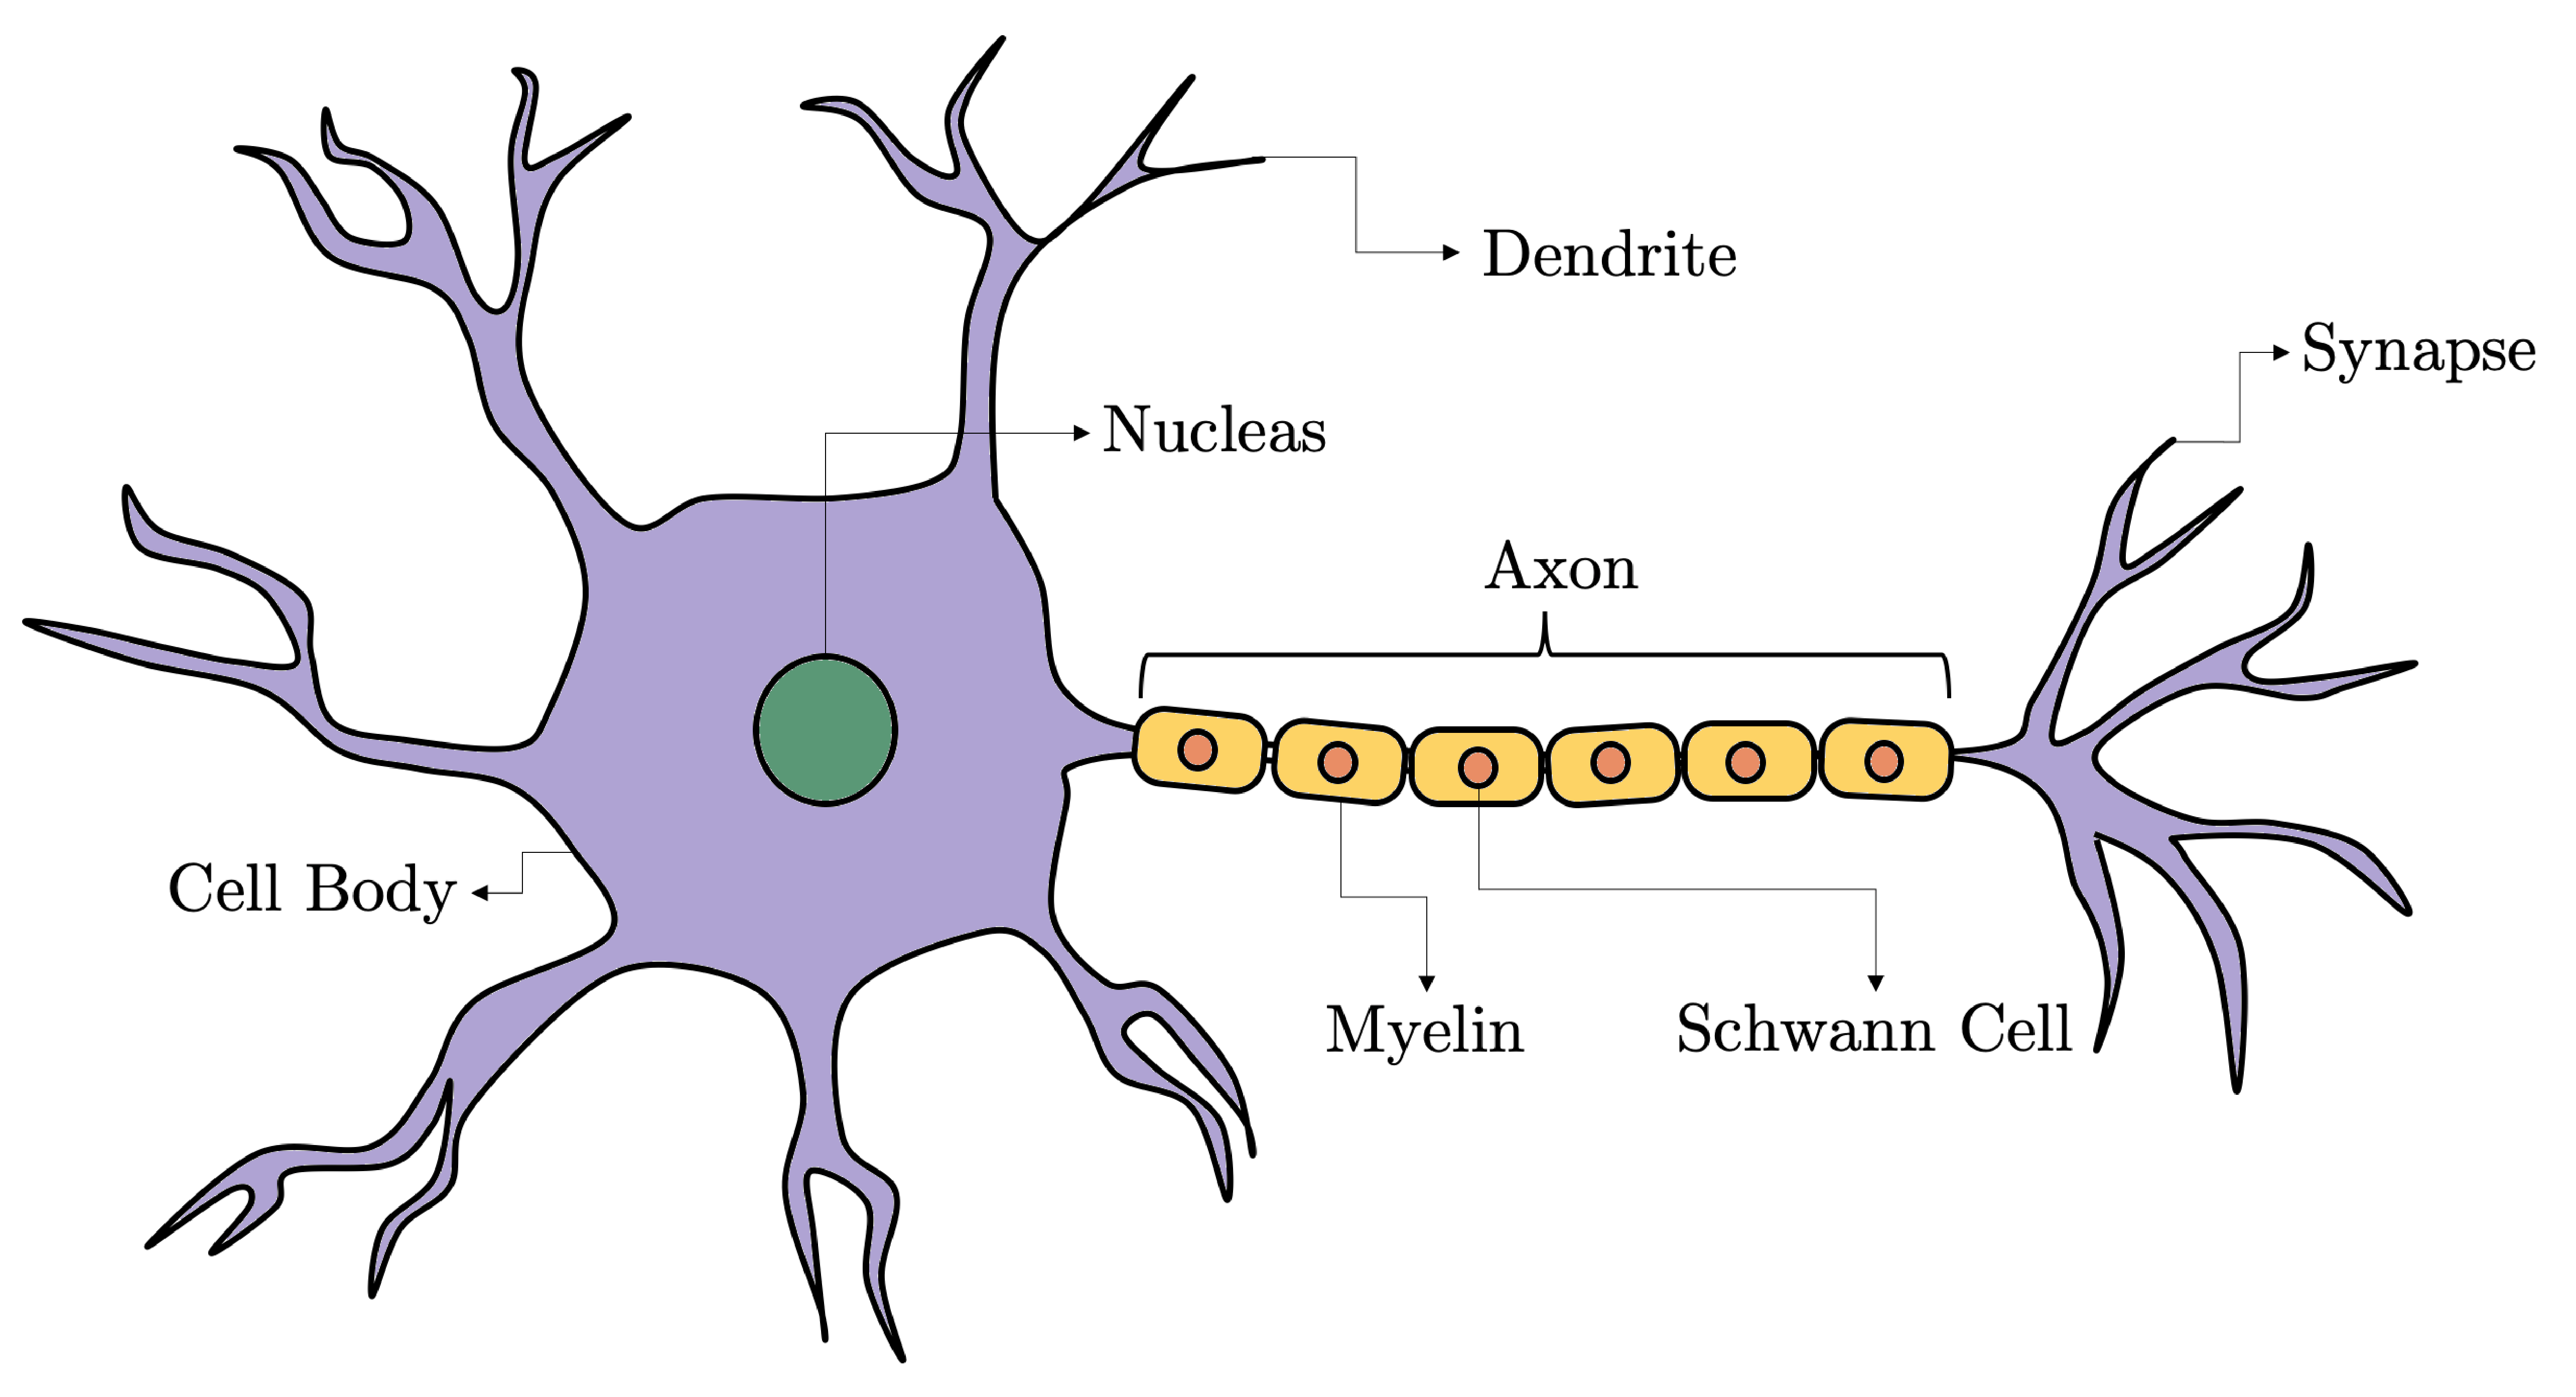
\includegraphics[width=0.8\textwidth]{biological_neuron.eps}
    \caption[The \index{Biological Neuron}Biological Neuron]{An illustration of
    the \index{Biological Neuron}Biological Neuron.}
    \label{fig:biological_neuron}
\end{figure}

The main parts of the \ac{BN} to focus on includes the cell body, the
\index{dendrites}\textit{dendrites} and the \index{axon}\textit{axon} because these
components are directly modeled in the \ac{AN}. \Acp{NN} are formed by
neurons that connect to each other. This is known as
\index{synaptogenesis}\textit{synaptogenesis} \cite{ref:huttenlocher:1997}.
Connections are made between the \index{axons}axons and
\index{dendrites}dendrites of various neurons. Such a connection is referred to
as a \index{synapse}\textit{synapse}. It is through \index{synapses}synapses
that neurons communicate with each other. Communication takes place by
electro-chemical pulse and is often referred to as an \textit{activation} or
\textit{action potential}.  Communication signals propagate from the
\index{dendrites}dendrites, through the cell body to the axon of a neuron,
provoking a signal in the post-synaptic neuron \cite{ref:engelbrecht:2007}.
Neurons like these are massively interconnected.  The greater the connection
between two neurons, the stronger the communication.  Kennedy
\cite{ref:kennedy:2016} defines stronger \index{Synapse}synapses as ones that
contribute more depolarisation to the neural membrane upon activation than
weaker ones. Stronger \index{Synapse}synapses have a higher probability of
generating an action potential in the post-synaptic neuron. During activation,
the pre-synaptic neuron release neurotransmitters that bind to the post-synaptic
neuron \cite{ref:khanacademy:synapse}. The frequent release of these molecules
cause the \index{synapse}synapse to grow. Connections that grow over time yield
stronger signals, while connections that are weak propagate low intensity
signals and vanish over time. This is how the human brain learns and forgets.
Every time we reinforce a memory in our brains, we ``train'' the neuron and the
connection becomes stronger. This is known as \index{synaptic
plasticity}\textit{synaptic plasticity} \cite{ref:huttenlocher:1997}. this
reinforcement of connections plays a pivotal role in the way we algorithmically
train \acp{ANN}.


\index{Artificial Neuron}
\section{Artificial Neuron}
\label{sec:anns:an}

This section introduces the \ac{AN}. It is shown how the \ac{AN} is modeled
after the \ac{BN} by providing a brief discussion on the various components that
make up the \ac{AN}. Each component is discussed in more detail, including input
modeling, weight modeling, \index{net input signal}net input signal modeling,
biases modeling and output modeling in the \ac{AN}.

\subsection{Components}
\label{sec:anns:components}

The An \ac{AN} implements a nonlinear mapping from $\mathbb{R}^{I}$ to
$\mathbb{R}^{T}$, usually in the ranges $[0,1]$ or $[-1,1]$, depending on the
activation function used \cite{ref:engelbrecht:2007}. This mapping is given
below:

\begin{equation}
    f_{AN} \colon \mathbb{R}^{I} \to \mathbb{R}^{T}
    \label{eq:an_function_mapping}
\end{equation}

\noindent
where $f_{AN}$ is the function mapping produced by the \ac{AN}, $I$
is the total number of dimensions of the input in real-number space $\mathbb{R}$
and $T$ is the total number of dimensions of the target (desired output) in
real-number space.

An illustration of the \ac{AN} is given below:

\begin{figure}[H]
  \centering
  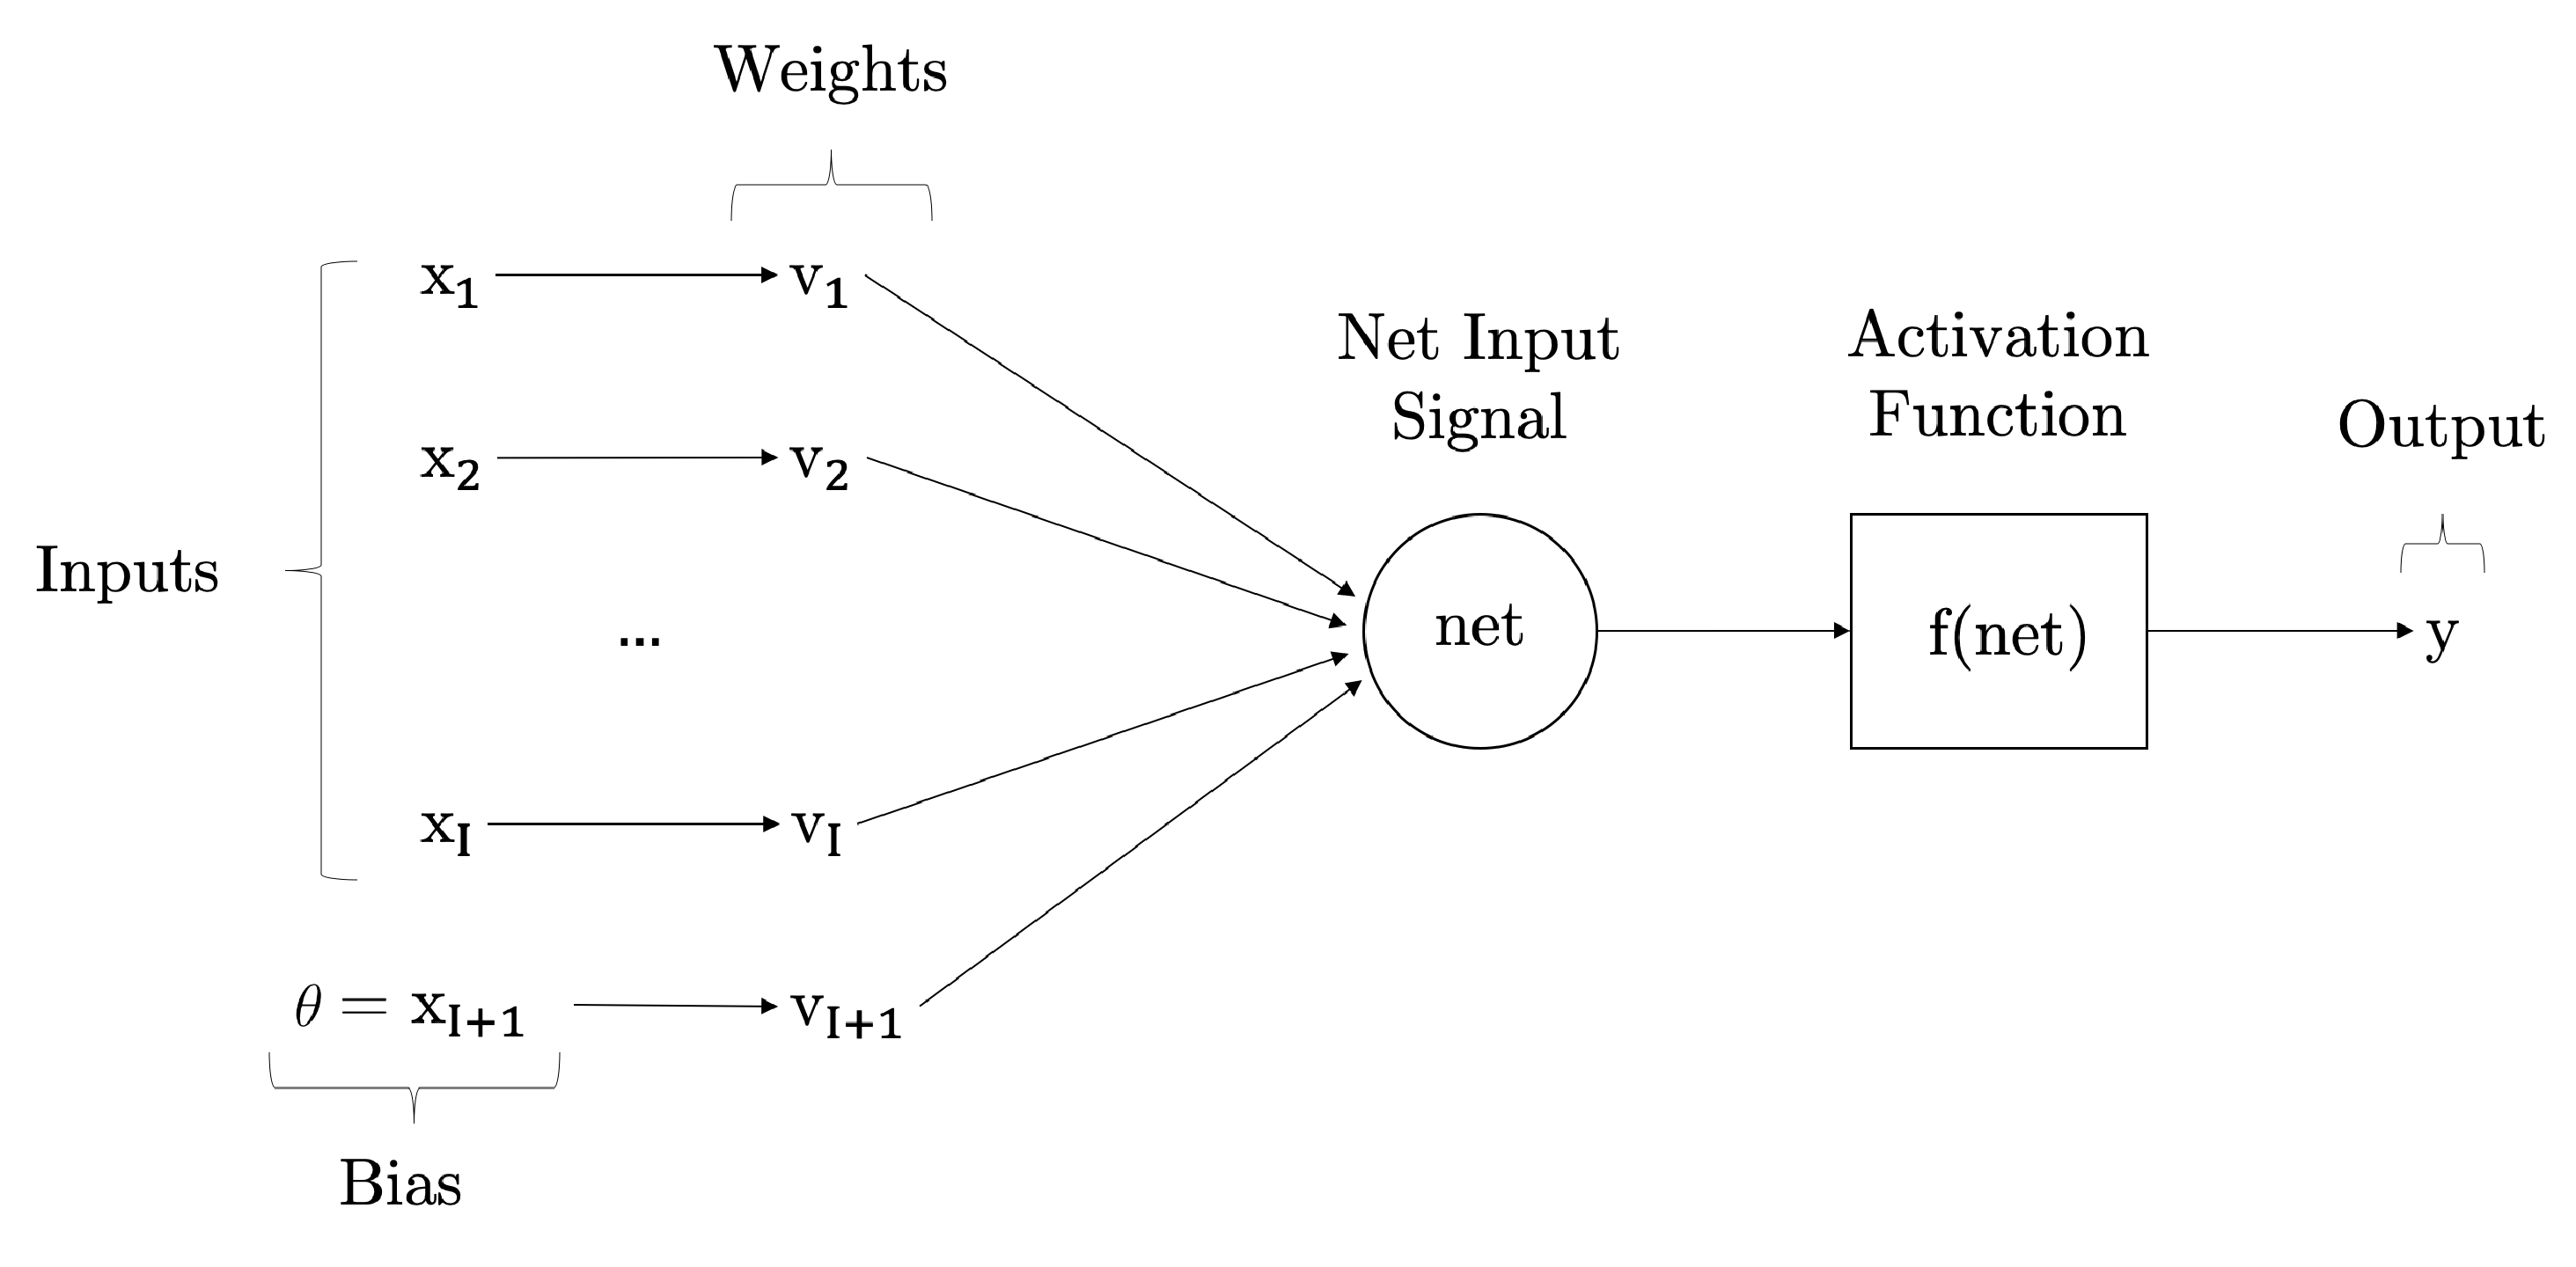
\includegraphics[width=\textwidth]{artificial_neuron.eps}
  \caption[The \index{Artificial Neuron}Artificial Neuron]{An illustration of
  the \index{Artificial Neuron}Artificial Neuron.}
  \label{fig:artificial_neuron}
\end{figure}

From Figure~\ref{fig:artificial_neuron}, one can see that the
\ac{AN} is made up of the following components:

\begin{itemize}
    \item
    \textbf{Input:} The input models the activations received from the pre-synaptic neuron
    or from some environment sensor. Input is represented by the input vector
    $\vec{x}$.

    \item
    \textbf{Weights:} The weights model the \index{synapse}synapses and connection
    strengths. Weights are represented by the weight vector, $\vec{v}$.

    \item
    \index{net input signal}\textbf{Net input signal:} The \index{net input signal}netinput signl models
    the net resulting activations from all connected pre-synaptic neurons or
    environment sensors. The \index{net input signal}net input signal is
    represented by $net$.

    \item
    \textbf{Biases:} The biases model a mechanism introduced to influence the strength of the
    activation (output signal) of the \index{AN}\ac{AN}. The bias is
    represented by $\theta$.

    \item
    \index{activation function}\textbf{Activation function:} Models the action potential of the
    \ac{BN}\index{BN} based on the net input signal. The \index{activation
    function}activation function is
    represented by $f$.

    \item
    \textbf{Output:} This output models the activation by the post-synaptic neuron. Output is
    represented by the output vector $\vec{y}$.
\end{itemize}

Each of the above mentioned components are discussed in detail in the following
sections.


\subsection{Input}
\label{sec:anns:an:input}

Input signals are $I$-dimensional vectors of numerical values that are obtained
either through some environment sensor or from other \acp{AN}. Input signals
are often referred to as \index{features}\textit{features} or \index{independent
variables}\textit{independent variables} \cite{ref:francis:2001}. In this
thesis, a single input vector is referred to as a pattern. Input data must first
be pre-processed before it is presented to the \ac{AN}. Input pre-processing
techniques are discussed next.


\subsubsection{Input Pre-processing}
\label{sec:anns:an:input:input_pre_processing}

Input pre-processing can help improve the training process, but also plays an
important role in determining the success of a practical application of the
\ac{ANN} \cite{ref:kuzniar:2017}. The primary purpose of input
pre-processing is to modify the input data so that it can better match predicted
output. 

There are many techniques to consider when pre-processing input data. From
scaling to the correct ranges to dealing with incomplete, invalid or even
irrelevant data. For the purposes of this thesis, only data encoding and
normalisation is considered. These topics are now discussed in more detail.


\index{Encoding}
\subsubsection{Encoding}
\label{sec:anns:an:input:encoding}

For qualitative data, such as class labels, the class labels have to be
converted to numerical representations. In general, class labels are encoded as
vectors \cite{ref:srinidhi:2018, ref:brownlee:2017:one-hot}. This thesis makes
use of \index{One-Hot Encoding}\textit{one-hot encoding} of class labels which
yields a $K$-dimensional output vector $\vec{y}$ of $0$'s and a single $1$. Each
element $y_k$ of $\vec{y}$ uniquely refers to a class. An activation, represented by a value
of $1$ at a given index thus represents a given class. Harris and Harris
\cite{ref:harris:2010} describe \index{One-Hot Encoding}one-hot encoding as a
group of vector elements where the representations of classes are represented
with a single high element (represented by $1$) and all the others low
(represented by $0$).

Once data has been encoded into the right form, normalisation is required. This
is discussed next.


\index{Normalisation}
\subsubsection{Normalisation}
\label{sec:anns:an:input:normalisation}

Input data must be normalised and scaled appropriately. In general, input data
is normalised to a range that is appropriate for the \index{Activation
Function}activation function being used. This yields input data in a range that
is comparable to the output produced. For the purpose of this thesis, the
min-max scaler \cite{ref:al:2006} and standard score scaler \cite{ref:jain:2005}
are normalisation techniques that are considered. These are discussed next.

\index{Min-Max Scalar}
\subsubsection{Min-Max Scaler}
\label{sec:anns:an:input:min_max_scaler}

The \index{Min-Max Scaler}min-max scaler scales all values into the range
$[0,1]$. This is also called \index{Unity-based
Normalisation}\textit{unity-based normalisation}. The
\index{min-max scaler}min-max scaler is used as a pre-processing technique for
target values when the \index{sigmoid}\textit{sigmoid} \index{activation
function} activation function is used and is given below:

\begin{equation}
    x_{i,p}'  = \frac{x_{i,p} - x_{i_{min}}}{x_{i_{max}} - x_{i_{min}}}
    \label{eq:min_max_scaler}
\end{equation}

\noindent where $x_{i,p}^{'}$ is the normalised form of $x_{i,p}$, the $i$-th
dimension of the input vector $\vec{x}_p$, $p \in \{1,2, \dots, P \}$, where $P$
is the total number of input patterns. $x_{i_{min}}$ and $x_{i_{max}}$ are
respectfully the minimum and maximum values of the $i$-th dimension for all
input vectors $\vec{x}_p, p \in \{1,2, \dots, P\}$.

\index{Standard Score Scalar}
\subsubsection{Standard Score Scaler}
\label{sec:anns:an:input:standard_score_scaler}

The \index{standard score scaler}standard score scaler, also known as the
\index{z-score scaler}\textit{z-score scaler}, scales features by subtracting
the mean and scaling to the unit variance of each dimension $i$ for all input
patterns $\vec{x}_p, p \in \{1,2, \dots, P\}$. The \index{standard score
scaler}standard score scaler is used as a pre-processing technique for target
values when the \index{hyperbolic tangent}\textit{hyperbolic tangent}
\index{activation function}activation function\index{activation function} is
used. The normalised for of $x_{i,p}^{'}$ as determined by the \index{standard
score scaler}standard score scaler is given in below: 

\begin{equation}
    x_{i,p}^{'} = \frac{x_{i,p} - \mu_i}{\sigma^2_i}
    \label{eq:standard_score_scaler}
\end{equation}

\noindent where $\mu_i$ and $\sigma^2_i$ are respectfully the mean and unit
variance of the $i$-th dimension of all input vectors $\vec{x}_p, p \in \{1,2,
\dots, P\}$.

\subsection{Weights}
\label{sec:anns:an:weights}

It was mentioned in Section~\ref{sec:anns:bn} that \index{synapses}synapses can
have strong or weak connections. The connection strength is modeled in the
\ac{AN} as weight vectors of numerical values associated with each dimension $i$
of the input data. Weights can either dampen or strengthen the input data by
some negative or positive numerical value. By changing the weight associated
with a feature, the influence of that particular feature on the predicted output
is changed. Finding the correct value for each weight, to yield optimal output,
is an optimisation problem \cite{ref:thierens:1993}. The initial placement of
these weight vectors in the search-space is very important. Research has shown
that weight initialisation plays an important role in the efficient training of
\acp{ANN} \cite{ref:thimm:1995}. Weight initialisation is discussed next,
followed by some common weight initialisation techniques used.

\index{Weight Initialisation}
\subsubsection{Weight Initialisation}
\label{sec:anns:an:weights:initialisation}

Weight initialisation is the process by which candidate solutions (represented
by the weights of the \ac{AN}) to the problem is placed in the search-space.
Weight initialisation influences the speed of convergence, the probability of
convergence and the generalisation capabilities of \acp{ANN}
\cite{ref:fernandez:2001}. Finding the optimal initialisation values for weights
is non-trivial and can be seen as another optimisation problem. Extensive
research on this topic has been done in the past \cite{ref:de:2016,
ref:erdogmus:2003, ref:yam:2000}.

\index{Weight Initialisation}Weight initialisation is dependent on the
\index{activation function}activation function used. If weights are initialised
to values that are too small, the vanishing gradients problem can occur
\cite{ref:hanin:2018}. If weights are initialised to values that are too big,
output of the activation function would not be in the active range. This leads
to hidden unit saturation and exploding gradients can occur
\cite{ref:hanin:2018, ref:yadav:2018}.

Research have presented many initialisation techniques \cite{ref:erdogmus:2003}.
Some techniques have been developed to address the problems that are mentioned
above \cite{ref:yadav:2018}. However, this thesis will only focus on
\index{random uniform sampling}random uniform sampling, \index{Glorot uniform
sampling}\textit{Glorot uniform (Xavier)} sampling and \index{Glorot normal
sampling}\textit{Glorot normal} sampling \cite{ref:glorot:2010}. These
techniques are briefly discussed next.


\index{random uniform sampling}
\subsubsection{Random Uniform Sampling}
\label{sec:anns:an:weights:random_uniform_sampling}

\index{random uniform sampling}Random uniform sampling initialises weights
uniformly in the range $[\omega_{min}, \omega_{max}]$, written as $w_{i} \sim
\textit{U} (\omega_{min}, \omega_{max})$ where the $\omega_{min}$ and
$\omega_{max}$ are respectfully the lower and upper bounds of the uniform
distribution. Suggested parameter values are $(-1, 1)$ or $(-0.5, 0.5)$
\cite{ref:nguyen:1990}.


\index{Glorot uniform sampling}
\subsubsection{Glorot Uniform Sampling}
\label{sec:anns:an:weights:glorot_uniform_sampling}

\index{Glorot uniform sampling}Glorot uniform sampling is a specialisation of
\index{random uniform sampling}random uniform sampling whereby $\omega =
\sqrt{\frac{6}{fanin + fanout}}$ and \index{$fanin$}$fanin$ is the number of
input neurons to the weight vector and \index{$fanout$}$fanout$ is the number of
output neurons from the weight vector.

\index{Glorot Normal Sampling}
\subsubsection{Glorot Normal Sampling}
\label{sec:anns:an:weights:glorot_normal_sampling}

\index{Glorot normal sampling}Glorot normal sampling initialises weights by
sampling from a truncated normal distribution centred on a mean of $0$ and with
$\sigma = \sqrt{\frac{2}{I + K}}$, where $\sigma$ is the standard deviation of
the distribution. $I$ and $K$ are respectfully the number of input and output
units in the weight vector. \index{Glorot normal sampling}Glorot normal sampling
have been shown to decrease training time \cite{ref:glorot:2010}.  


\index{net input signal}
\subsection{Net Input Signal}
\label{sec:anns:an:net_input}

\acp{AN} accumulate the net resulting input signal from all input dimensions
into a value called the \index{net input signal}\textit{net input signal},
expressed as $net$. This signal is passed to the \index{Activation
Function}activation function, which provokes an artificial action potential in
the \ac{AN}.

The most common way by which the \index{net input signal}net input signal is
calculated is by means of \acp{SU} \cite{ref:engelbrecht:2007}, which
computes the \index{net input signal}net input signal as the weighted sum of all
input signals as shown below:

\begin{equation}
    net = \sum_{i=1}^{I}{x_{i}v_{i}}
    \label{eq:summation_units}
\end{equation}

\noindent where $x_{i}$ is the $i$-th
dimension of the input vector $\vec{x}$, and $v_{i}$ is the $i$-th dimension of
the weight vector $\vec{v}$, associated with the given input dimension. 


\subsection{Biases}
\label{sec:anns:an:biases}

A bias/threshold term $\theta$ is introduced to help translate the output of the
\index{activation function}activation function \cite{ref:benitez:1997}. The
value of $\theta$ must be learned during the training process along with the
weights of the \ac{ANN}. In order to simplify equations, augmented vectors are
used in which input and hidden layers have an additional neuron/unit, called the
\textit{bias unit} \cite{ref:engelbrecht:2007}. Augumented vectors that include
the bias unit to the net input signal is presented next.


\subsubsection{Augmented Net Input Signal}
\label{sec:anns:an:biases:augmented_net_input_signal}

Input layer $x_{I+1}$ has a net input signal $net^{'} = net - \theta$. The value
for $\theta$ is learned along with the weights such that $\theta =
x_{i+1}v_{i+1}$. If a constant value $x_{i+1} = -1$ is used, the equation for
\acp{SU} as given in Equation~\eqref{eq:summation_units} is then completed by
including $\theta$ as shown below:

\begin{equation}
    \begin{split}
        net{'} & = net - \theta \\
             & = \sum_{i=1}^{I} x_i v_i - \theta\\
             & = \sum_{i=1}^{I} x_i v_i + x_{i+1} v_{i+1} \\
             & = \sum_{i=1}^{I+1} x_i v_i
    \label{eq:augmented_vectors}
    \end{split}
\end{equation}

\noindent where $\textit{net}^{'}$ is the augmented net input signal that now
includes the bias term $\theta$.


\subsection{Activation Functions}
\label{sec:anns:an:act_functions}

\index{activation function}Activation functions are used to model the action
potential of the \index{AN}\ac{AN} \cite{ref:ziv:1994, ref:hodgkin:1952}, and is
a function over the augmented \index{net input signal}net input signal. It is
the mechanism that models whether an \index{AN}\ac{AN} fires or not. When the
output produced by the activation function surpasses some threshold value
$\theta$, we consider that neuron to have fired an output signal.
\index{activation function}Activation functions model \textit{phase shift}. In
the context of classification problems, these \index{activation
function}activation functions form decision boundaries between classes. In the
context of regression problems, these \index{activation function}activation
functions try to approximate some function that maps the input data to some
target data.

In general, activation functions produce a non-linear mapping of
$\mathbb{R}^{I}$ to the range $[0,1]$ or $[-1,1]$ as shown below:

\begin{equation}
    f_{AN}: \mathbb{R}^{I} \rightarrow [0,1]
    \label{eq:an_function_mapping_0_1}
\end{equation}

\noindent or

\begin{equation}
    f_{AN}: \mathbb{R}^{I} \rightarrow [-1,1]
    \label{eq:an_function_mapping_minus_1_1}
\end{equation}

\noindent Research in the past have presented many \index{activation
function}activation functions \cite{ref:karlik:2011} of varying ranges. However,
this thesis focuses on the \ac{ReLU} \cite{ref:jarrett:2009, ref:nair:2010}, the
\ac{LReLU} \cite{ref:maas:2013}, the \index{sigmoid}sigmoid \cite{ref:lecun:1988} and the
\index{hyperbolic tangent}hyperbolic tangent \cite{ref:lin:2008} \index{activation
function}activation functions. These \index{activation function}activation
functions are presented next.


\subsubsection{Rectified Linear Unit}
\label{sec:anns:an:act_functions:relu}

The \ac{ReLU} \index{activation function}activation function is an
\index{activation function}activation function defined in the positive part of
its argument. It is defined as:

\begin{equation}
    f(x) = x^{+} = \max(0,x)
    \label{eq:relu}
\end{equation}

\noindent An advantage of \ac{ReLU} is that it is not susceptible to the
\index{vanishing gradient problem}vanishing gradients problem \cite{ref:xu:2015,
ref:maksutov:2018} which occurs when gradients in the first layers of a
multi-layer \ac{ANN} approach zero, and have no effect in the training process.


\subsubsection{Leaky Rectified Linear Unit}
\label{sec:anns:an:act_functions:leaky_relu}

The \ac{LReLU} \index{activation function}activation function is a variant of
the \ac{ReLU} \index{activation function}activation function \cite{ref:xu:2015}.
Similar to \ac{ReLU} it is not susceptible to the \index{vanishing gradients
problem}vanishing gradients problem and it does not suffer from the \index{dying
ReLU problem}dying \ac{ReLU} problem \cite{ref:agarap:2018}, which occurs when
the neurons that use \ac{ReLU} \index{activation functions}activation functions
become \textit{inactive} and only output $0$ due to a negative net input signal.

The \ac{LReLU} \index{activation function}activation function is defines as:
	
\begin{equation}
    f_{AN}(net - \theta) = 
    \begin{cases}
        net - \theta & \text{if $net \geq \theta $}\\
        \alpha(net - \theta) & \text{otherwise}\\
    \end{cases}
    \label{eq:leaky_relu}
\end{equation}

\noindent
By introducing a parameter $\alpha >
0$, negative \index{Net Input Signals}net input signals will still yield
non-zero activations, resulting in non-zero gradients and avoiding gradient
saturation. Non-zero gradients are required by some heuristics such as
\ac{SGD} in order to be able to effectively train \acp{ANN}
\cite{ref:hanin:2018}.

An illustration of the \ac{LReLU} with various values for $\alpha$ and $\theta =
0$ is given in Graph~\ref{grf:leaky_relu} below:

\begin{graph}[H]
    \centering
    % GNUPLOT: LaTeX picture with Postscript
\begingroup
  \makeatletter
  \providecommand\color[2][]{%
    \GenericError{(gnuplot) \space\space\space\@spaces}{%
      Package color not loaded in conjunction with
      terminal option `colourtext'%
    }{See the gnuplot documentation for explanation.%
    }{Either use 'blacktext' in gnuplot or load the package
      color.sty in LaTeX.}%
    \renewcommand\color[2][]{}%
  }%
  \providecommand\includegraphics[2][]{%
    \GenericError{(gnuplot) \space\space\space\@spaces}{%
      Package graphicx or graphics not loaded%
    }{See the gnuplot documentation for explanation.%
    }{The gnuplot epslatex terminal needs graphicx.sty or graphics.sty.}%
    \renewcommand\includegraphics[2][]{}%
  }%
  \providecommand\rotatebox[2]{#2}%
  \@ifundefined{ifGPcolor}{%
    \newif\ifGPcolor
    \GPcolorfalse
  }{}%
  \@ifundefined{ifGPblacktext}{%
    \newif\ifGPblacktext
    \GPblacktexttrue
  }{}%
  % define a \g@addto@macro without @ in the name:
  \let\gplgaddtomacro\g@addto@macro
  % define empty templates for all commands taking text:
  \gdef\gplbacktext{}%
  \gdef\gplfronttext{}%
  \makeatother
  \ifGPblacktext
    % no textcolor at all
    \def\colorrgb#1{}%
    \def\colorgray#1{}%
  \else
    % gray or color?
    \ifGPcolor
      \def\colorrgb#1{\color[rgb]{#1}}%
      \def\colorgray#1{\color[gray]{#1}}%
      \expandafter\def\csname LTw\endcsname{\color{white}}%
      \expandafter\def\csname LTb\endcsname{\color{black}}%
      \expandafter\def\csname LTa\endcsname{\color{black}}%
      \expandafter\def\csname LT0\endcsname{\color[rgb]{1,0,0}}%
      \expandafter\def\csname LT1\endcsname{\color[rgb]{0,1,0}}%
      \expandafter\def\csname LT2\endcsname{\color[rgb]{0,0,1}}%
      \expandafter\def\csname LT3\endcsname{\color[rgb]{1,0,1}}%
      \expandafter\def\csname LT4\endcsname{\color[rgb]{0,1,1}}%
      \expandafter\def\csname LT5\endcsname{\color[rgb]{1,1,0}}%
      \expandafter\def\csname LT6\endcsname{\color[rgb]{0,0,0}}%
      \expandafter\def\csname LT7\endcsname{\color[rgb]{1,0.3,0}}%
      \expandafter\def\csname LT8\endcsname{\color[rgb]{0.5,0.5,0.5}}%
    \else
      % gray
      \def\colorrgb#1{\color{black}}%
      \def\colorgray#1{\color[gray]{#1}}%
      \expandafter\def\csname LTw\endcsname{\color{white}}%
      \expandafter\def\csname LTb\endcsname{\color{black}}%
      \expandafter\def\csname LTa\endcsname{\color{black}}%
      \expandafter\def\csname LT0\endcsname{\color{black}}%
      \expandafter\def\csname LT1\endcsname{\color{black}}%
      \expandafter\def\csname LT2\endcsname{\color{black}}%
      \expandafter\def\csname LT3\endcsname{\color{black}}%
      \expandafter\def\csname LT4\endcsname{\color{black}}%
      \expandafter\def\csname LT5\endcsname{\color{black}}%
      \expandafter\def\csname LT6\endcsname{\color{black}}%
      \expandafter\def\csname LT7\endcsname{\color{black}}%
      \expandafter\def\csname LT8\endcsname{\color{black}}%
    \fi
  \fi
    \setlength{\unitlength}{0.0500bp}%
    \ifx\gptboxheight\undefined%
      \newlength{\gptboxheight}%
      \newlength{\gptboxwidth}%
      \newsavebox{\gptboxtext}%
    \fi%
    \setlength{\fboxrule}{0.5pt}%
    \setlength{\fboxsep}{1pt}%
\begin{picture}(7200.00,5040.00)%
    \gplgaddtomacro\gplbacktext{%
      \csname LTb\endcsname%%
      \put(3545,2652){\makebox(0,0)[r]{\strut{}}}%
      \put(3545,484){\makebox(0,0)[r]{\strut{}$-1$}}%
      \put(3545,1568){\makebox(0,0)[r]{\strut{}$-0.5$}}%
      \put(3545,3735){\makebox(0,0)[r]{\strut{}$0.5$}}%
      \put(3545,4819){\makebox(0,0)[r]{\strut{}$1$}}%
      \put(3677,2369){\makebox(0,0){\strut{}}}%
      \put(550,2369){\makebox(0,0){\strut{}$-1$}}%
      \put(2113,2369){\makebox(0,0){\strut{}$-0.5$}}%
      \put(5240,2369){\makebox(0,0){\strut{}$0.5$}}%
      \put(6803,2369){\makebox(0,0){\strut{}$1$}}%
    }%
    \gplgaddtomacro\gplfronttext{%
      \csname LTb\endcsname%%
      \put(77,2651){\rotatebox{-270}{\makebox(0,0){\strut{}$f_{AN}(net - \theta)$}}}%
      \put(3676,154){\makebox(0,0){\strut{}$net - \theta$}}%
      \csname LTb\endcsname%%
      \put(1606,4536){\makebox(0,0)[r]{\strut{}$\alpha=0.0$}}%
      \csname LTb\endcsname%%
      \put(1606,4316){\makebox(0,0)[r]{\strut{}$\alpha=0.1$}}%
      \csname LTb\endcsname%%
      \put(1606,4096){\makebox(0,0)[r]{\strut{}$\alpha=0.3$}}%
      \csname LTb\endcsname%%
      \put(1606,3876){\makebox(0,0)[r]{\strut{}$\alpha=0.5$}}%
    }%
    \gplbacktext
    \put(0,0){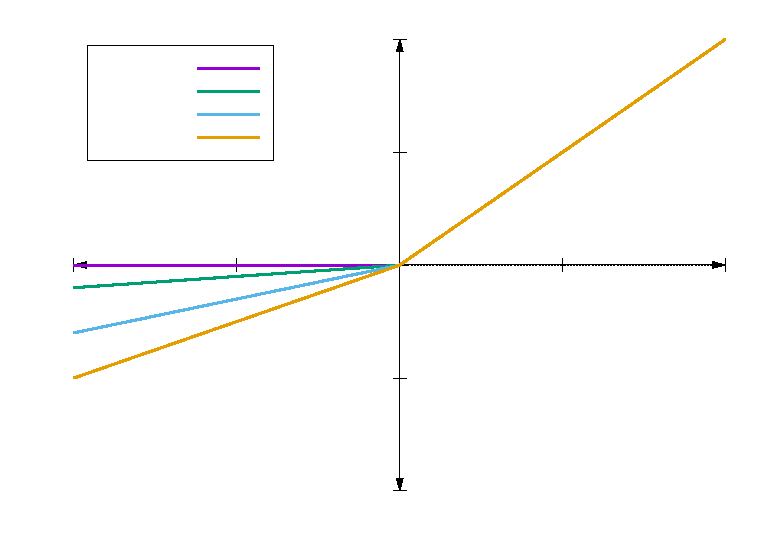
\includegraphics[width={360.00bp},height={252.00bp}]{leaky_relu}}%
    \gplfronttext
  \end{picture}%
\endgroup

    \caption[The \ac{LReLU} \index{activation function}activation function]{An illustration of the
    \acs{LReLU} \index{activation function}activation function.}
    \label{grf:leaky_relu}
\end{graph}


\subsubsection{Sigmoid}
\label{sec:anns:an:act_functions:sigmoid}

\index{sigmoid}Sigmoid is a very popular \index{activation function}activation
function, because it introduces non-linearity into the model. The
\index{sigmoid}sigmoid \index{activation function}activation function is defined
as:
	
\begin{equation}
    f_{AN}(net - \theta) = \frac{1}{1+e^{-\lambda(net - \theta)}}
    \label{eq:sigmoid}
\end{equation}

\noindent where $\lambda$ is a control parameter, which controls the steepness
of the function and is usually set to $\lambda = 1$.  \noindent The
\index{sigmoid}sigmoid \index{activation function}activation function is a
continuous variant of the ramp function and yields $f_{AN} \in (0,1)$.

An illustration of the \index{sigmoid}sigmoid \index{Activation
Function}activation function with various values for $\lambda$ and $\theta = 0$
is given below:

\begin{graph}[H]
    \centering
    \resizebox{0.8\textwidth}{!}{% GNUPLOT: LaTeX picture with Postscript
\begingroup
  \makeatletter
  \providecommand\color[2][]{%
    \GenericError{(gnuplot) \space\space\space\@spaces}{%
      Package color not loaded in conjunction with
      terminal option `colourtext'%
    }{See the gnuplot documentation for explanation.%
    }{Either use 'blacktext' in gnuplot or load the package
      color.sty in LaTeX.}%
    \renewcommand\color[2][]{}%
  }%
  \providecommand\includegraphics[2][]{%
    \GenericError{(gnuplot) \space\space\space\@spaces}{%
      Package graphicx or graphics not loaded%
    }{See the gnuplot documentation for explanation.%
    }{The gnuplot epslatex terminal needs graphicx.sty or graphics.sty.}%
    \renewcommand\includegraphics[2][]{}%
  }%
  \providecommand\rotatebox[2]{#2}%
  \@ifundefined{ifGPcolor}{%
    \newif\ifGPcolor
    \GPcolorfalse
  }{}%
  \@ifundefined{ifGPblacktext}{%
    \newif\ifGPblacktext
    \GPblacktexttrue
  }{}%
  % define a \g@addto@macro without @ in the name:
  \let\gplgaddtomacro\g@addto@macro
  % define empty templates for all commands taking text:
  \gdef\gplbacktext{}%
  \gdef\gplfronttext{}%
  \makeatother
  \ifGPblacktext
    % no textcolor at all
    \def\colorrgb#1{}%
    \def\colorgray#1{}%
  \else
    % gray or color?
    \ifGPcolor
      \def\colorrgb#1{\color[rgb]{#1}}%
      \def\colorgray#1{\color[gray]{#1}}%
      \expandafter\def\csname LTw\endcsname{\color{white}}%
      \expandafter\def\csname LTb\endcsname{\color{black}}%
      \expandafter\def\csname LTa\endcsname{\color{black}}%
      \expandafter\def\csname LT0\endcsname{\color[rgb]{1,0,0}}%
      \expandafter\def\csname LT1\endcsname{\color[rgb]{0,1,0}}%
      \expandafter\def\csname LT2\endcsname{\color[rgb]{0,0,1}}%
      \expandafter\def\csname LT3\endcsname{\color[rgb]{1,0,1}}%
      \expandafter\def\csname LT4\endcsname{\color[rgb]{0,1,1}}%
      \expandafter\def\csname LT5\endcsname{\color[rgb]{1,1,0}}%
      \expandafter\def\csname LT6\endcsname{\color[rgb]{0,0,0}}%
      \expandafter\def\csname LT7\endcsname{\color[rgb]{1,0.3,0}}%
      \expandafter\def\csname LT8\endcsname{\color[rgb]{0.5,0.5,0.5}}%
    \else
      % gray
      \def\colorrgb#1{\color{black}}%
      \def\colorgray#1{\color[gray]{#1}}%
      \expandafter\def\csname LTw\endcsname{\color{white}}%
      \expandafter\def\csname LTb\endcsname{\color{black}}%
      \expandafter\def\csname LTa\endcsname{\color{black}}%
      \expandafter\def\csname LT0\endcsname{\color{black}}%
      \expandafter\def\csname LT1\endcsname{\color{black}}%
      \expandafter\def\csname LT2\endcsname{\color{black}}%
      \expandafter\def\csname LT3\endcsname{\color{black}}%
      \expandafter\def\csname LT4\endcsname{\color{black}}%
      \expandafter\def\csname LT5\endcsname{\color{black}}%
      \expandafter\def\csname LT6\endcsname{\color{black}}%
      \expandafter\def\csname LT7\endcsname{\color{black}}%
      \expandafter\def\csname LT8\endcsname{\color{black}}%
    \fi
  \fi
    \setlength{\unitlength}{0.0500bp}%
    \ifx\gptboxheight\undefined%
      \newlength{\gptboxheight}%
      \newlength{\gptboxwidth}%
      \newsavebox{\gptboxtext}%
    \fi%
    \setlength{\fboxrule}{0.5pt}%
    \setlength{\fboxsep}{1pt}%
\begin{picture}(7200.00,5040.00)%
    \gplgaddtomacro\gplbacktext{%
      \csname LTb\endcsname%%
      \put(3545,878){\makebox(0,0)[r]{\strut{}}}%
      \put(3545,1666){\makebox(0,0)[r]{\strut{}$0.2$}}%
      \put(3545,2454){\makebox(0,0)[r]{\strut{}$0.4$}}%
      \put(3545,3243){\makebox(0,0)[r]{\strut{}$0.6$}}%
      \put(3545,4031){\makebox(0,0)[r]{\strut{}$0.8$}}%
      \put(3545,4819){\makebox(0,0)[r]{\strut{}$1$}}%
      \put(3677,595){\makebox(0,0){\strut{}}}%
      \put(1175,595){\makebox(0,0){\strut{}$-4$}}%
      \put(2426,595){\makebox(0,0){\strut{}$-2$}}%
      \put(4927,595){\makebox(0,0){\strut{}$2$}}%
      \put(6178,595){\makebox(0,0){\strut{}$4$}}%
    }%
    \gplgaddtomacro\gplfronttext{%
      \csname LTb\endcsname%%
      \put(77,2651){\rotatebox{-270}{\makebox(0,0){\strut{}$f_{AN}(net - \theta)$}}}%
      \put(3676,154){\makebox(0,0){\strut{}$net - \theta$}}%
      \csname LTb\endcsname%%
      \put(1342,4536){\makebox(0,0)[r]{\strut{}$\lambda=1$}}%
      \csname LTb\endcsname%%
      \put(1342,4316){\makebox(0,0)[r]{\strut{}$\lambda=3$}}%
      \csname LTb\endcsname%%
      \put(1342,4096){\makebox(0,0)[r]{\strut{}$\lambda=5$}}%
      \csname LTb\endcsname%%
      \put(1342,3876){\makebox(0,0)[r]{\strut{}$\lambda=8$}}%
    }%
    \gplbacktext
    \put(0,0){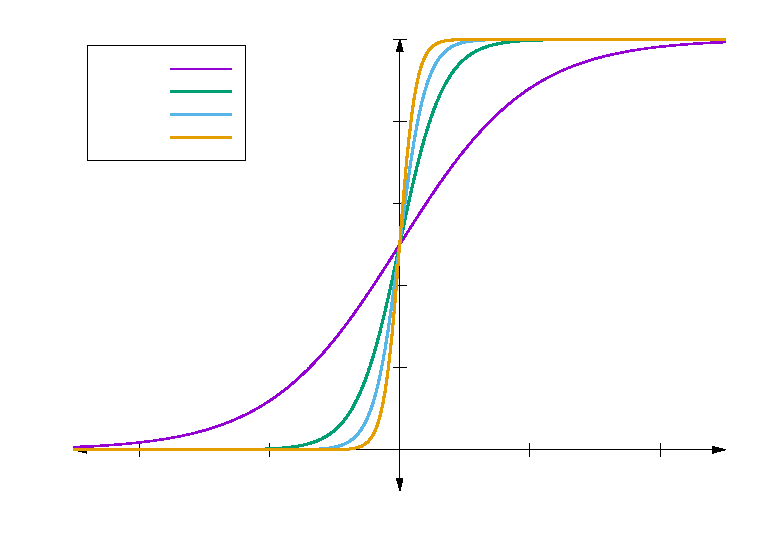
\includegraphics[width={360.00bp},height={252.00bp}]{sigmoid}}%
    \gplfronttext
  \end{picture}%
\endgroup
}
    \caption[The \index{sigmoid}sigmoid \index{activation function}activation
    function]{An illustration of the \index{sigmoid}sigmoid \index{Activation
    Function}activation function.}
    \label{grf:sigmoid}
\end{graph}


\subsubsection{Hyperbolic Tangent}
\label{sec:anns:an:act_functions:tanh}

The \index{hyperbolic tangent}hyperbolic tangent \index{activation
function}activation function is similar to the \index{sigmoid}sigmoid
\index{activation function}activation function, but yields output in the range
$(-1, 1)$. The \index{hyperbolic tangent}hyperbolic tangent
\index{activation function}activation function is defined as:
	
\begin{equation}
    f_{AN}(net - \theta) = \frac{e^{\lambda(net - \theta)}-e^{-\lambda(net - \theta)}}{e^{\lambda(net - \theta)}+e^{-\lambda(net - \theta)}}
    \label{eq:hyperbolic_tangent}
\end{equation}

\noindent The \index{hyperbolic tangent}hyperbolic tangent \index{activation
function}activation function with various values for $\lambda$ and $\theta = 0$
is given below:

\begin{graph}[H]
    \centering
    \resizebox{0.8\textwidth}{!}{% GNUPLOT: LaTeX picture with Postscript
\begingroup
  \makeatletter
  \providecommand\color[2][]{%
    \GenericError{(gnuplot) \space\space\space\@spaces}{%
      Package color not loaded in conjunction with
      terminal option `colourtext'%
    }{See the gnuplot documentation for explanation.%
    }{Either use 'blacktext' in gnuplot or load the package
      color.sty in LaTeX.}%
    \renewcommand\color[2][]{}%
  }%
  \providecommand\includegraphics[2][]{%
    \GenericError{(gnuplot) \space\space\space\@spaces}{%
      Package graphicx or graphics not loaded%
    }{See the gnuplot documentation for explanation.%
    }{The gnuplot epslatex terminal needs graphicx.sty or graphics.sty.}%
    \renewcommand\includegraphics[2][]{}%
  }%
  \providecommand\rotatebox[2]{#2}%
  \@ifundefined{ifGPcolor}{%
    \newif\ifGPcolor
    \GPcolorfalse
  }{}%
  \@ifundefined{ifGPblacktext}{%
    \newif\ifGPblacktext
    \GPblacktexttrue
  }{}%
  % define a \g@addto@macro without @ in the name:
  \let\gplgaddtomacro\g@addto@macro
  % define empty templates for all commands taking text:
  \gdef\gplbacktext{}%
  \gdef\gplfronttext{}%
  \makeatother
  \ifGPblacktext
    % no textcolor at all
    \def\colorrgb#1{}%
    \def\colorgray#1{}%
  \else
    % gray or color?
    \ifGPcolor
      \def\colorrgb#1{\color[rgb]{#1}}%
      \def\colorgray#1{\color[gray]{#1}}%
      \expandafter\def\csname LTw\endcsname{\color{white}}%
      \expandafter\def\csname LTb\endcsname{\color{black}}%
      \expandafter\def\csname LTa\endcsname{\color{black}}%
      \expandafter\def\csname LT0\endcsname{\color[rgb]{1,0,0}}%
      \expandafter\def\csname LT1\endcsname{\color[rgb]{0,1,0}}%
      \expandafter\def\csname LT2\endcsname{\color[rgb]{0,0,1}}%
      \expandafter\def\csname LT3\endcsname{\color[rgb]{1,0,1}}%
      \expandafter\def\csname LT4\endcsname{\color[rgb]{0,1,1}}%
      \expandafter\def\csname LT5\endcsname{\color[rgb]{1,1,0}}%
      \expandafter\def\csname LT6\endcsname{\color[rgb]{0,0,0}}%
      \expandafter\def\csname LT7\endcsname{\color[rgb]{1,0.3,0}}%
      \expandafter\def\csname LT8\endcsname{\color[rgb]{0.5,0.5,0.5}}%
    \else
      % gray
      \def\colorrgb#1{\color{black}}%
      \def\colorgray#1{\color[gray]{#1}}%
      \expandafter\def\csname LTw\endcsname{\color{white}}%
      \expandafter\def\csname LTb\endcsname{\color{black}}%
      \expandafter\def\csname LTa\endcsname{\color{black}}%
      \expandafter\def\csname LT0\endcsname{\color{black}}%
      \expandafter\def\csname LT1\endcsname{\color{black}}%
      \expandafter\def\csname LT2\endcsname{\color{black}}%
      \expandafter\def\csname LT3\endcsname{\color{black}}%
      \expandafter\def\csname LT4\endcsname{\color{black}}%
      \expandafter\def\csname LT5\endcsname{\color{black}}%
      \expandafter\def\csname LT6\endcsname{\color{black}}%
      \expandafter\def\csname LT7\endcsname{\color{black}}%
      \expandafter\def\csname LT8\endcsname{\color{black}}%
    \fi
  \fi
    \setlength{\unitlength}{0.0500bp}%
    \ifx\gptboxheight\undefined%
      \newlength{\gptboxheight}%
      \newlength{\gptboxwidth}%
      \newsavebox{\gptboxtext}%
    \fi%
    \setlength{\fboxrule}{0.5pt}%
    \setlength{\fboxsep}{1pt}%
\begin{picture}(7200.00,5040.00)%
    \gplgaddtomacro\gplbacktext{%
      \csname LTb\endcsname%%
      \put(3545,2652){\makebox(0,0)[r]{\strut{}}}%
      \put(3545,484){\makebox(0,0)[r]{\strut{}$-1$}}%
      \put(3545,1568){\makebox(0,0)[r]{\strut{}$-0.5$}}%
      \put(3545,3735){\makebox(0,0)[r]{\strut{}$0.5$}}%
      \put(3545,4819){\makebox(0,0)[r]{\strut{}$1$}}%
      \put(3677,2369){\makebox(0,0){\strut{}}}%
      \put(550,2369){\makebox(0,0){\strut{}$-1$}}%
      \put(2113,2369){\makebox(0,0){\strut{}$-0.5$}}%
      \put(5240,2369){\makebox(0,0){\strut{}$0.5$}}%
      \put(6803,2369){\makebox(0,0){\strut{}$1$}}%
    }%
    \gplgaddtomacro\gplfronttext{%
      \csname LTb\endcsname%%
      \put(77,2651){\rotatebox{-270}{\makebox(0,0){\strut{}$f_{AN}(net - \theta)$}}}%
      \put(3676,154){\makebox(0,0){\strut{}$net - \theta$}}%
      \csname LTb\endcsname%%
      \put(1342,4536){\makebox(0,0)[r]{\strut{}$\lambda=1$}}%
      \csname LTb\endcsname%%
      \put(1342,4316){\makebox(0,0)[r]{\strut{}$\lambda=3$}}%
      \csname LTb\endcsname%%
      \put(1342,4096){\makebox(0,0)[r]{\strut{}$\lambda=5$}}%
      \csname LTb\endcsname%%
      \put(1342,3876){\makebox(0,0)[r]{\strut{}$\lambda=8$}}%
    }%
    \gplbacktext
    \put(0,0){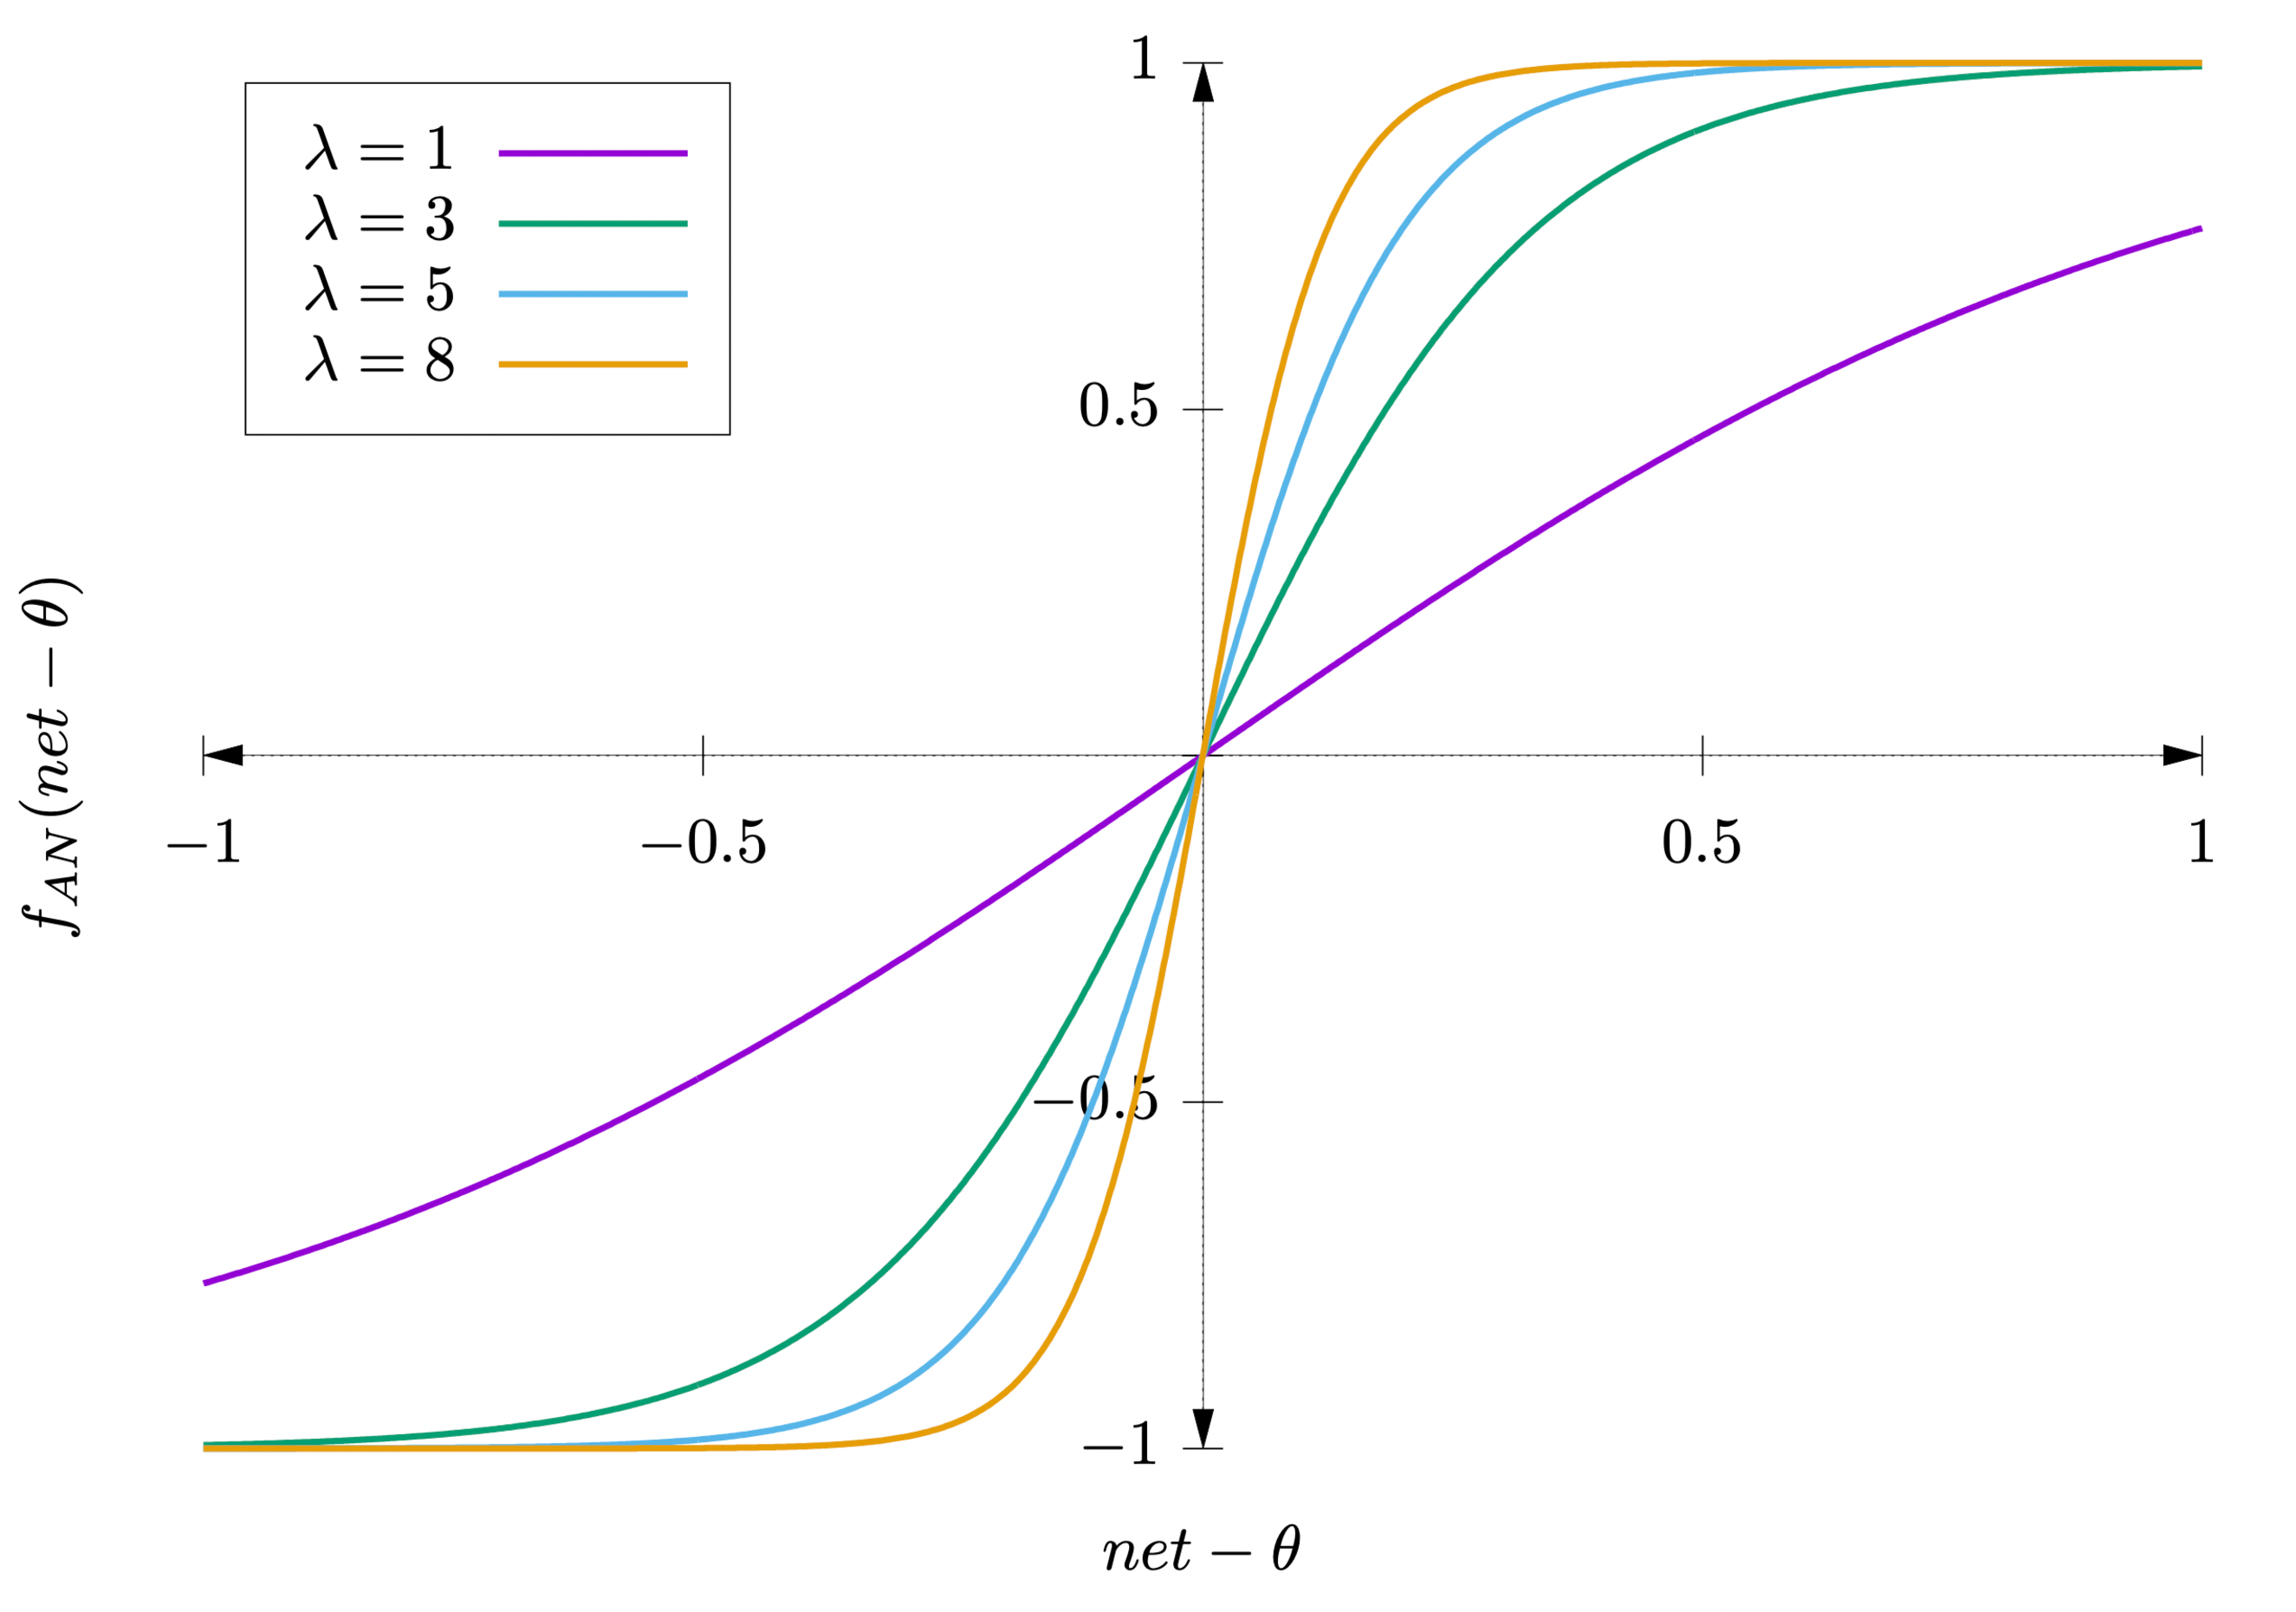
\includegraphics[width={360.00bp},height={252.00bp}]{tanh}}%
    \gplfronttext
  \end{picture}%
\endgroup
}
    \vspace{10pt}
    \caption[The \index{hyperbolic tangent}hyperbolic tangent \index{Activation
        Function}activation function]{An illustration of the \index{Hyperbolic
    Tangent}hyperbolic tangent \index{activation function}activation function.}
    \label{grf:hyperbolic_tangent}
\end{graph}


\subsection{Output}
\label{sec:anns:an:output}

Output signals are $K$-dimensional vectors of numerical values that are produced
by the \index{activation function}activation function. Output signals are often
referred to as \textit{predictions}. If target pre-processing was applied, it is
necessary to post-process the output data. A brief discussion on post-processing
techniques follow.

\subsubsection{Output Post-Processing}
\label{sec:anns:an:output:output_post_processing}

Output post-processing is necessary in order to convert data back to their
original ranges. The post-processing techniques that are applicable depend on
the type of problem (regression or classification), input pre-processing
techniques used, as well as the \index{activation function}activation function
used. For the purposes of this thesis, only data decoding, normalisation and
re-scaling techniques are considered.


\subsubsection{Decoding}
\label{sec:anns:an:output:decoding}

Data decoding is used to convert \index{One-Hot Encoding}one-hot encoded vectors
as described in Section~\ref{sec:anns:an:input:encoding} back to class labels.
This is relevant to classification problems where the predicted output is a
\index{One-Hot Encoding}one-hot encoded vector representing a class label.

The high value (represented by $1$) at $y_k$ is used to decode the
\index{One-Hot Encoding}one-hot encoded output vector $\vec{y}$ back to its
corresponding class label.

Normalisation of the output data is used to simplify the decoding process. This
thesis considers \index{softmax}\textit{softmax} and
\index{Argmax}\textit{argmax} normalisation to assist the decoding process.


\subsubsection{Softmax}
\label{sec:anns:an:output:softmax}

The \index{softmax}softmax function, also known as the
\index{softargmax}\textit{softargmax} \cite[p.~184]{ref:goodfellow:2016} or
\index{normalised exponential function}\textit{normalised exponential function}
\cite{ref:bishop:2006} is a generalisation of the logistic function that
converts the $K$-dimensional output vector $\vec{y}$ into a $K$-dimensional
output vector $\vec{y^{'}}$ where each element $y^{'}_k$ is in the range $(0,1)$
and all elements sum up to $1$. This is expressed as follows:

\begin{equation}
    \vec{y^{'}} \colon \mathbb{R}^{K} \to \left\{\vec{y^{'}} \in \mathbb{R}^{K} \vert y^{'}_k \in (0,1), \sum_{k=1}^{K} y_k = 1\right\}
    \label{eq:sum_after_softmax}
\end{equation}

\noindent The softmax function is given as:

\begin{equation}
    y^{'}_k = \frac{e^{y_k}}{\sum_{k = 1}^{K}e^{y_k}}
    \label{eq:softmax}
\end{equation}


\subsubsection{Argmax}
\label{sec:anns:an:output:argmax}

The \index{Argmax}argmax function is similar to the \index{softmax}softmax
function, with the difference that the element $y_k, k \in \{1,2, \dots, K\}$
with the highest output value is set to $1$ and the rest are set to $0$. This
means that all elements still sum to $1$, but the activation is only observed at
index $k$ where the activation is $1$.

The \index{Argmax}argmax function is given as:

\begin{equation}
    y^{'}_k = 
    \begin{cases}
        1 & \text{if $y_k = \max(y_1, y_2, \dots, y_K)$}\\
        0 & \text{otherwise}
        \label{eq:argmax}
    \end{cases}
\end{equation}

\noindent Graph~\ref{grf:softmax_argmax} illustrates the comparison of
transformations of the output vector $\vec{y}$, where the
\index{sigmoid}sigmoid, the \index{softmax}softmax and the \index{argmax}argmax
\index{activation function}activation functions are used.


\begin{graph}[H]
    \centering
    \resizebox{0.8\textwidth}{!}{% GNUPLOT: LaTeX picture with Postscript
\begingroup
  \makeatletter
  \providecommand\color[2][]{%
    \GenericError{(gnuplot) \space\space\space\@spaces}{%
      Package color not loaded in conjunction with
      terminal option `colourtext'%
    }{See the gnuplot documentation for explanation.%
    }{Either use 'blacktext' in gnuplot or load the package
      color.sty in LaTeX.}%
    \renewcommand\color[2][]{}%
  }%
  \providecommand\includegraphics[2][]{%
    \GenericError{(gnuplot) \space\space\space\@spaces}{%
      Package graphicx or graphics not loaded%
    }{See the gnuplot documentation for explanation.%
    }{The gnuplot epslatex terminal needs graphicx.sty or graphics.sty.}%
    \renewcommand\includegraphics[2][]{}%
  }%
  \providecommand\rotatebox[2]{#2}%
  \@ifundefined{ifGPcolor}{%
    \newif\ifGPcolor
    \GPcolorfalse
  }{}%
  \@ifundefined{ifGPblacktext}{%
    \newif\ifGPblacktext
    \GPblacktexttrue
  }{}%
  % define a \g@addto@macro without @ in the name:
  \let\gplgaddtomacro\g@addto@macro
  % define empty templates for all commands taking text:
  \gdef\gplbacktext{}%
  \gdef\gplfronttext{}%
  \makeatother
  \ifGPblacktext
    % no textcolor at all
    \def\colorrgb#1{}%
    \def\colorgray#1{}%
  \else
    % gray or color?
    \ifGPcolor
      \def\colorrgb#1{\color[rgb]{#1}}%
      \def\colorgray#1{\color[gray]{#1}}%
      \expandafter\def\csname LTw\endcsname{\color{white}}%
      \expandafter\def\csname LTb\endcsname{\color{black}}%
      \expandafter\def\csname LTa\endcsname{\color{black}}%
      \expandafter\def\csname LT0\endcsname{\color[rgb]{1,0,0}}%
      \expandafter\def\csname LT1\endcsname{\color[rgb]{0,1,0}}%
      \expandafter\def\csname LT2\endcsname{\color[rgb]{0,0,1}}%
      \expandafter\def\csname LT3\endcsname{\color[rgb]{1,0,1}}%
      \expandafter\def\csname LT4\endcsname{\color[rgb]{0,1,1}}%
      \expandafter\def\csname LT5\endcsname{\color[rgb]{1,1,0}}%
      \expandafter\def\csname LT6\endcsname{\color[rgb]{0,0,0}}%
      \expandafter\def\csname LT7\endcsname{\color[rgb]{1,0.3,0}}%
      \expandafter\def\csname LT8\endcsname{\color[rgb]{0.5,0.5,0.5}}%
    \else
      % gray
      \def\colorrgb#1{\color{black}}%
      \def\colorgray#1{\color[gray]{#1}}%
      \expandafter\def\csname LTw\endcsname{\color{white}}%
      \expandafter\def\csname LTb\endcsname{\color{black}}%
      \expandafter\def\csname LTa\endcsname{\color{black}}%
      \expandafter\def\csname LT0\endcsname{\color{black}}%
      \expandafter\def\csname LT1\endcsname{\color{black}}%
      \expandafter\def\csname LT2\endcsname{\color{black}}%
      \expandafter\def\csname LT3\endcsname{\color{black}}%
      \expandafter\def\csname LT4\endcsname{\color{black}}%
      \expandafter\def\csname LT5\endcsname{\color{black}}%
      \expandafter\def\csname LT6\endcsname{\color{black}}%
      \expandafter\def\csname LT7\endcsname{\color{black}}%
      \expandafter\def\csname LT8\endcsname{\color{black}}%
    \fi
  \fi
    \setlength{\unitlength}{0.0500bp}%
    \ifx\gptboxheight\undefined%
      \newlength{\gptboxheight}%
      \newlength{\gptboxwidth}%
      \newsavebox{\gptboxtext}%
    \fi%
    \setlength{\fboxrule}{0.5pt}%
    \setlength{\fboxsep}{1pt}%
\begin{picture}(7200.00,5040.00)%
    \gplgaddtomacro\gplbacktext{%
      \csname LTb\endcsname%%
      \put(814,704){\makebox(0,0)[r]{\strut{}$0$}}%
      \put(814,1253){\makebox(0,0)[r]{\strut{}$0.2$}}%
      \put(814,1801){\makebox(0,0)[r]{\strut{}$0.4$}}%
      \put(814,2350){\makebox(0,0)[r]{\strut{}$0.6$}}%
      \put(814,2899){\makebox(0,0)[r]{\strut{}$0.8$}}%
      \put(814,3447){\makebox(0,0)[r]{\strut{}$1$}}%
      \put(814,3996){\makebox(0,0)[r]{\strut{}$1.2$}}%
      \put(814,4545){\makebox(0,0)[r]{\strut{}$1.4$}}%
      \put(1532,484){\makebox(0,0){\strut{}$y_{1}$}}%
      \put(2703,484){\makebox(0,0){\strut{}$y_{2}$}}%
      \put(3875,484){\makebox(0,0){\strut{}$y_{3}$}}%
      \put(5046,484){\makebox(0,0){\strut{}$y_{4}$}}%
      \put(6217,484){\makebox(0,0){\strut{}$y_{5}$}}%
    }%
    \gplgaddtomacro\gplfronttext{%
      \csname LTb\endcsname%%
      \put(209,2761){\rotatebox{-270}{\makebox(0,0){\strut{}Activation}}}%
      \put(3874,154){\makebox(0,0){\strut{}Output Dimension}}%
      \csname LTb\endcsname%%
      \put(5816,4536){\makebox(0,0)[r]{\strut{}Sigmoid}}%
      \csname LTb\endcsname%%
      \put(5816,4316){\makebox(0,0)[r]{\strut{}Softmax}}%
      \csname LTb\endcsname%%
      \put(5816,4096){\makebox(0,0)[r]{\strut{}Argmax}}%
      \csname LTb\endcsname%%
      \put(1239,3695){\rotatebox{90}{\makebox(0,0){\strut{}0.97}}}%
      \put(2410,1665){\rotatebox{90}{\makebox(0,0){\strut{}0.23}}}%
      \put(3582,1336){\rotatebox{90}{\makebox(0,0){\strut{}0.11}}}%
      \put(4753,1895){\rotatebox{90}{\makebox(0,0){\strut{}0.31}}}%
      \put(5924,1171){\rotatebox{90}{\makebox(0,0){\strut{}0.05}}}%
      \put(1532,1994){\rotatebox{90}{\makebox(0,0){\strut{}0.35}}}%
      \put(2703,1500){\rotatebox{90}{\makebox(0,0){\strut{}0.17}}}%
      \put(3875,1446){\rotatebox{90}{\makebox(0,0){\strut{}0.15}}}%
      \put(5046,1528){\rotatebox{90}{\makebox(0,0){\strut{}0.18}}}%
      \put(6217,1418){\rotatebox{90}{\makebox(0,0){\strut{}0.14}}}%
      \put(1825,3777){\rotatebox{90}{\makebox(0,0){\strut{}1.00}}}%
      \put(2996,1034){\rotatebox{90}{\makebox(0,0){\strut{}0.00}}}%
      \put(4167,1034){\rotatebox{90}{\makebox(0,0){\strut{}0.00}}}%
      \put(5339,1034){\rotatebox{90}{\makebox(0,0){\strut{}0.00}}}%
      \put(6510,1034){\rotatebox{90}{\makebox(0,0){\strut{}0.00}}}%
    }%
    \gplbacktext
    \put(0,0){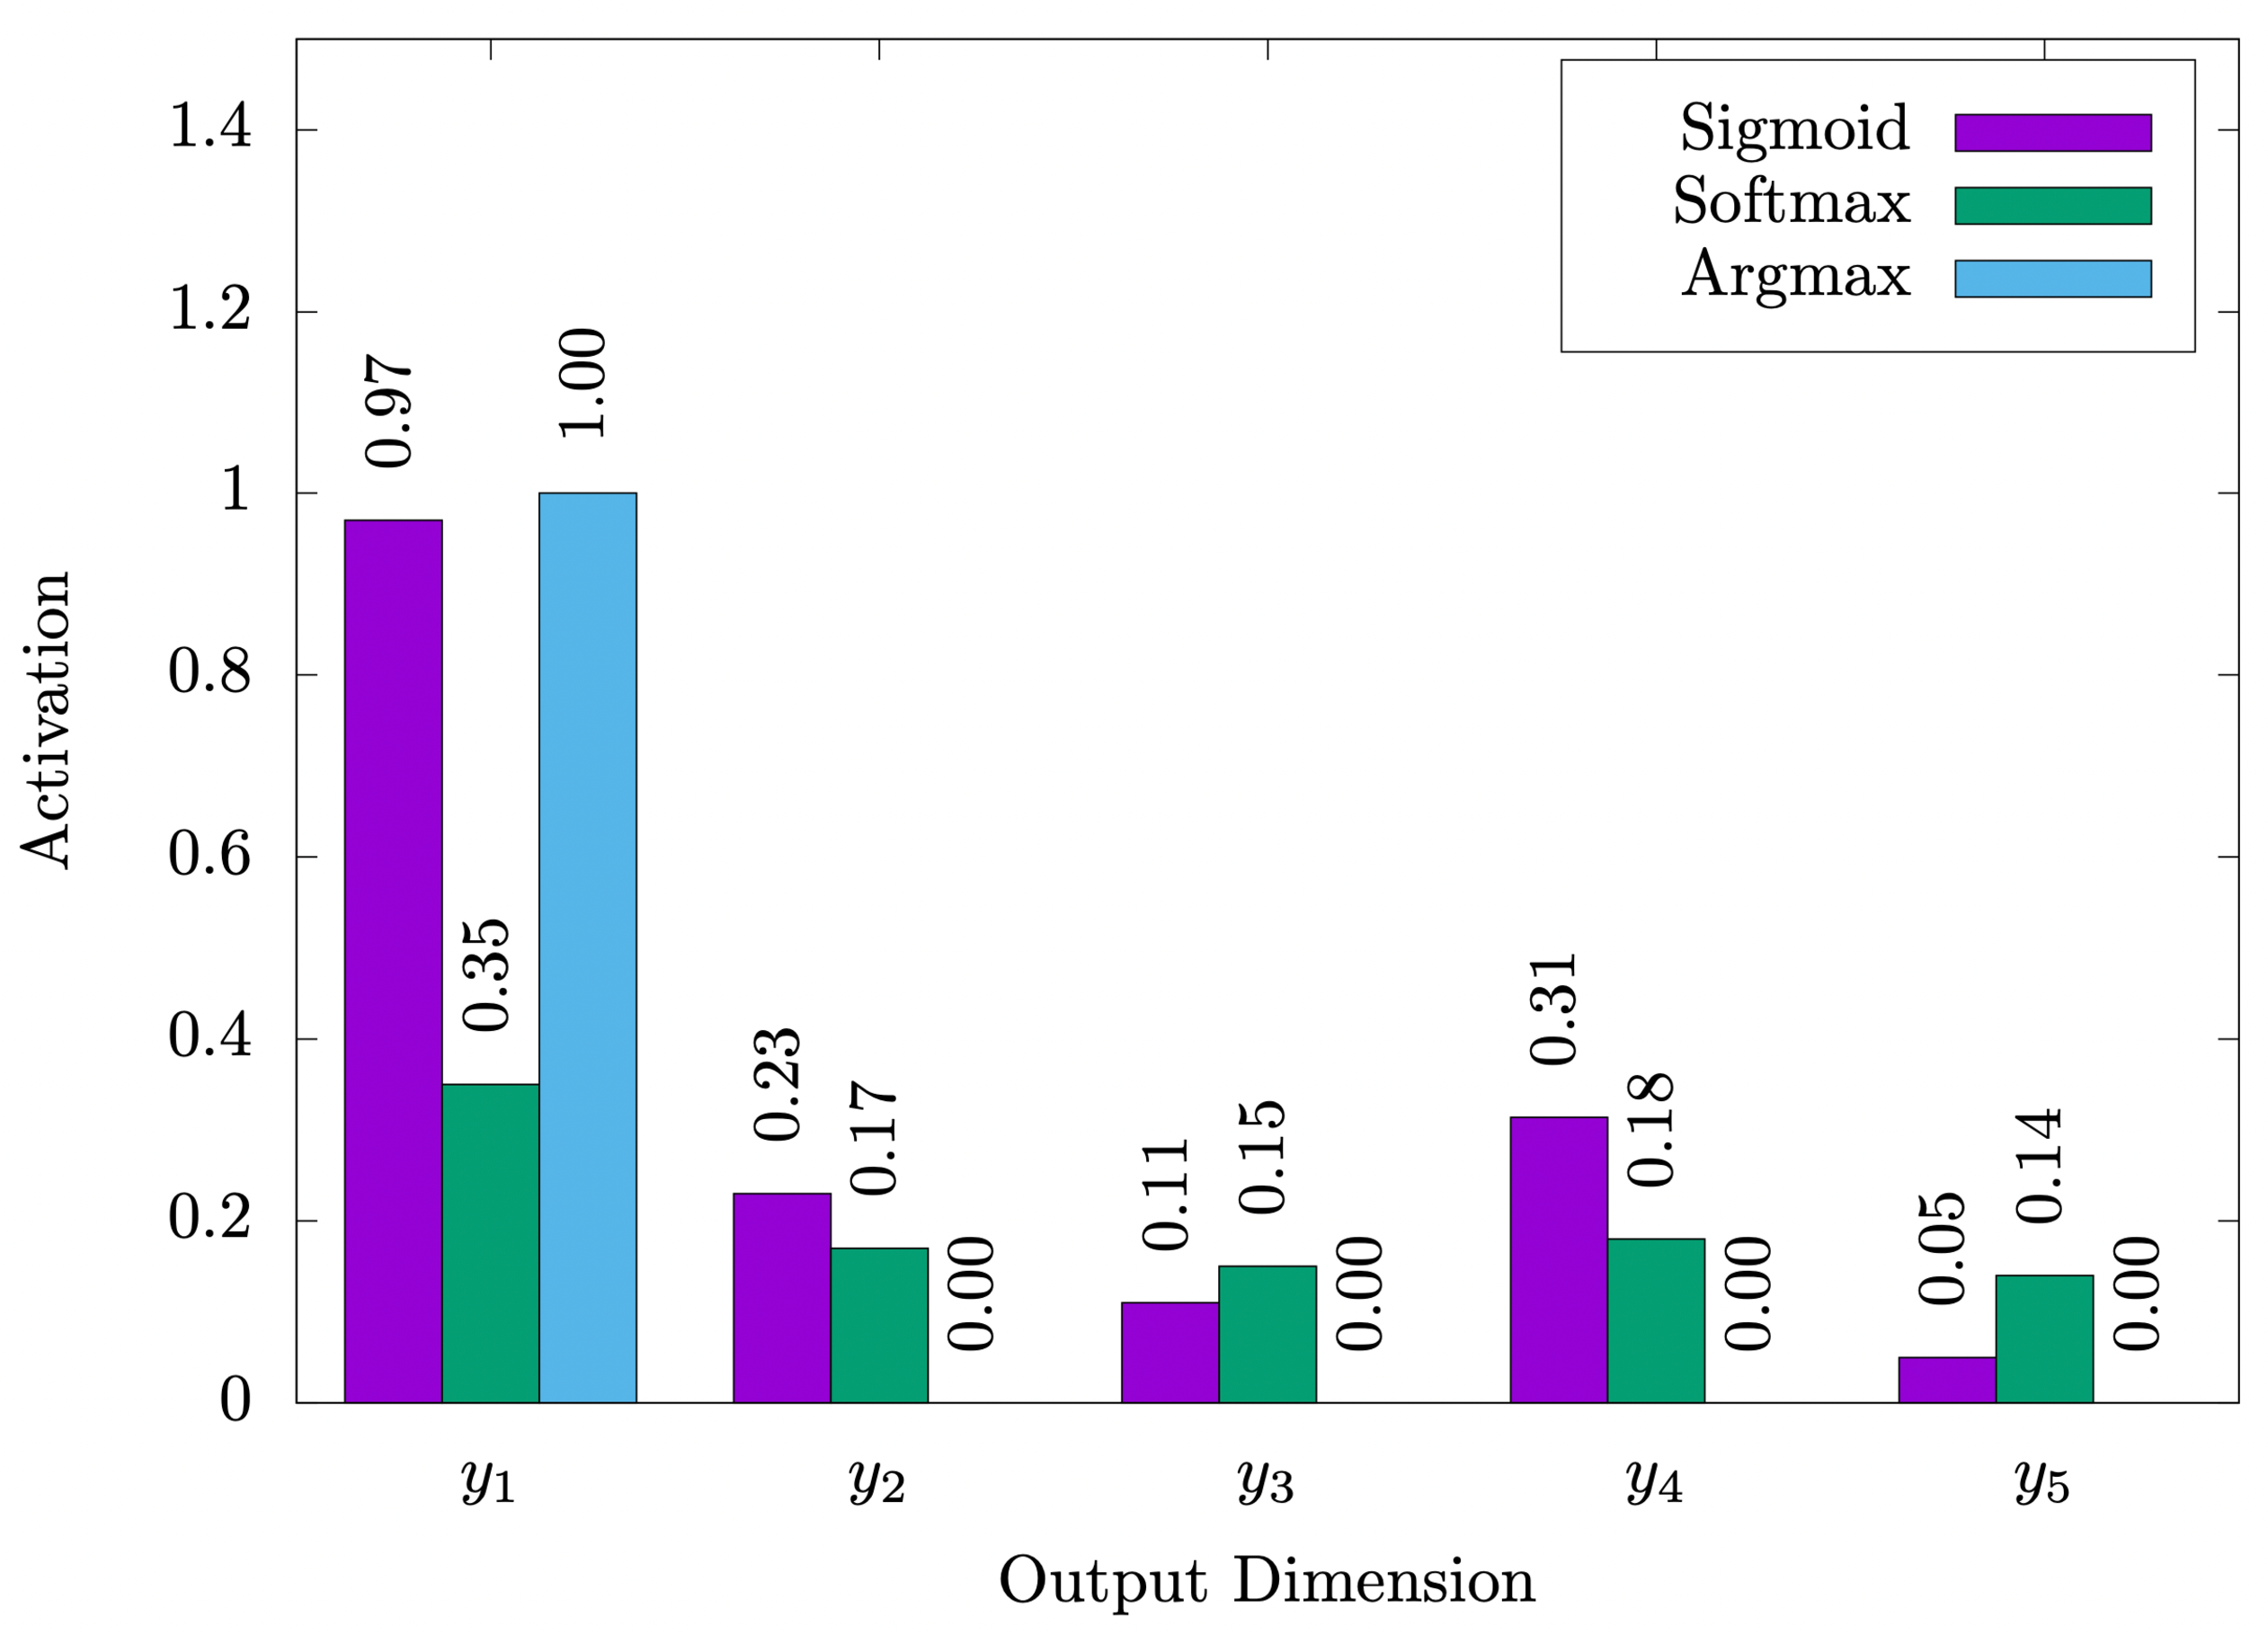
\includegraphics[width={360.00bp},height={252.00bp}]{output_modifiers}}%
    \gplfronttext
  \end{picture}%
\endgroup
}
    \caption[The results of \index{softmax}softmax and \index{Argmax}argmax]{An
        illustration of \index{softmax}softmax and \index{Argmax}argmax applied
    after the \index{sigmoid}sigmoid \index{activation function}activation function.}
    \label{grf:softmax_argmax}
\end{graph}


\section{Artificial Neural Network}
\label{sec:anns:ann}

This section presents \acp{ANN}. Discussions follow on their applications,
architecture, and topologies. Finally, a specific type of \ac{ANN} called a
\acl{FFNN} is discussed in detail.

\subsection{Applications}
\label{sec:anns:anns:applications}

\acp{ANN} are modelled after our biological brains. The human brain is
biologically and chemically incredibly sophisticated. Trying to model an entire
brain is at this stage not computationally feasible. Sandberg
\cite{ref:sandberg:2008} approximates a computational requirement of 256 000
terabytes/s to emulate the entire brain. Given our shortage in hardware
capabilities, \acp{ANN} have been successfully applied to a range of problem
classes. Engelbrecht \cite{ref:engelbrecht:2007} summarises some common problems
that are solved using \acp{ANN}. These include: 

\begin{itemize}
    \item
    \textbf{Classification}: Predicting the class of an input vector
    \cite{ref:khan:2001}.
    
    \item
    \textbf{Pattern Matching}: Producing closely associated patterns based on an
    input vector \cite{ref:cannady:1998, ref:kumar:1994}.
    
    \item
    \textbf{Pattern Completion}: Completing the missing parts of an input vector
    \cite{ref:dayhoff:2001}.

    \item
    \textbf{Optimisation}: Producing optimal values of parameters in a
    optimisation problems \cite{ref:specht:1991}.

    \item
    \textbf{Data Mining}: Feature discovery in large datasets
    \cite{ref:singh:2009}.
\end{itemize}

Different \acp{ANN} are built for different types of problems, however, most
applications of \acp{ANN} include some layered architecture. Discussions follow
on \ac{ANN} architecture and topologies.

\subsection{Architecture}
\label{sec:anns:anns:architecture}

\acp{ANN} are collections of \acp{AN} that are organised together to form a
connected network. The architecture of the \ac{ANN} refers to the way in which
these \acp{AN} are organised together as well as the type of \index{Activation
Function}activation function used.

\acp{ANN} are organised in layers where a single layer can contain multiple
\acp{AN}. Generally, each layer makes use of the same \index{activation
function}activation function, but this is not a requirement. Output from one
layer is propagated as input to the next layer. This thesis focusses on the
simplest architecture, containing three particular layers, including the input,
hidden and output layers. \acp{ANN} with this type of architecture is usually
referred to as \textit{shallow} \acp{NN}. The input, hidden and output layers
are discussed next.

The input layer contains the input data to the \ac{ANN}. Since the
input layer simply provides the the input data, some literature do not consider
the input layer as a layer \cite{ref:engelbrecht:2007}.

The hidden layer contains a collection of hidden \acp{AN}. These hidden \acp{AN}
are referred to as \textit{hidden units} or \textit{nodes}. Hidden units are
used if the target data is not linearly separable \cite{ref:engelbrecht:2007}.
It has been shown that \acp{ANN} that incorporate monotonically increasing
differentiable \index{activation function}activation functions can approximate
any continuous function with just one hidden layer, given that the hidden layer
has enough hidden units \cite{ref:hornik:1989}. 

The output layer contains the activations or the predictions of the \ac{ANN}.
This layer is used to analyse the accuracy of the prediction and thus the
performance of the \ac{ANN}.


\subsection{Topology}
\label{sec:anns:anns:topology}

The topology of the \ac{ANN} refers to the way \acp{AN} are connected to each
other. Since \acp{AN} are organised in layers, this connectivity is described
layer by layer.

There are many different topologies \cite{ref:miikkulainen:2010}, however, this
thesis only focusses on a \index{fully connected topology}fully connected
topology.

The most common and simplest topology is where each \ac{AN} in one layer is
connected to all \acp{AN} in the next. Fully connected topologies have no
cycles \cite{ref:zell:1994}.


\subsection{Feedforward Neural Networks}
\label{sec:anns:anns:ffnns}

There are many different types of \acp{ANN}. All \acp{ANN} can be described
in terms of their architecture and topology. This research will focus on a
particular \ac{ANN} called a \acl{FFNN} (\acs{FFNN}).

\acp{FFNN} were the first and simplest \acp{ANN} developed
\cite{ref:schmidhuber:2015}. \acp{FFNN} incorporate the basic layers (input,
hidden and output layers) by arranging them in sequential order. In \acp{FFNN}
information moves forward, in one direction, from the input nodes, through the
hidden nodes and finally to the output nodes and depending on the optimisation
algorith used, error correction information can be backpropagated through the
network. It can be said that input is \textit{fed} forward, through the
\ac{ANN}. The \index{activation function}activation function used is problem
dependent. \acp{FFNN} incorporate fully connected topologies amongst the layers
such that no cycles form \cite{ref:zell:1994}.

An illustration of a \ac{FFNN} using a three-layered architecture and a fully
connected topology is given below:

\begin{figure}[H]
    \centering
    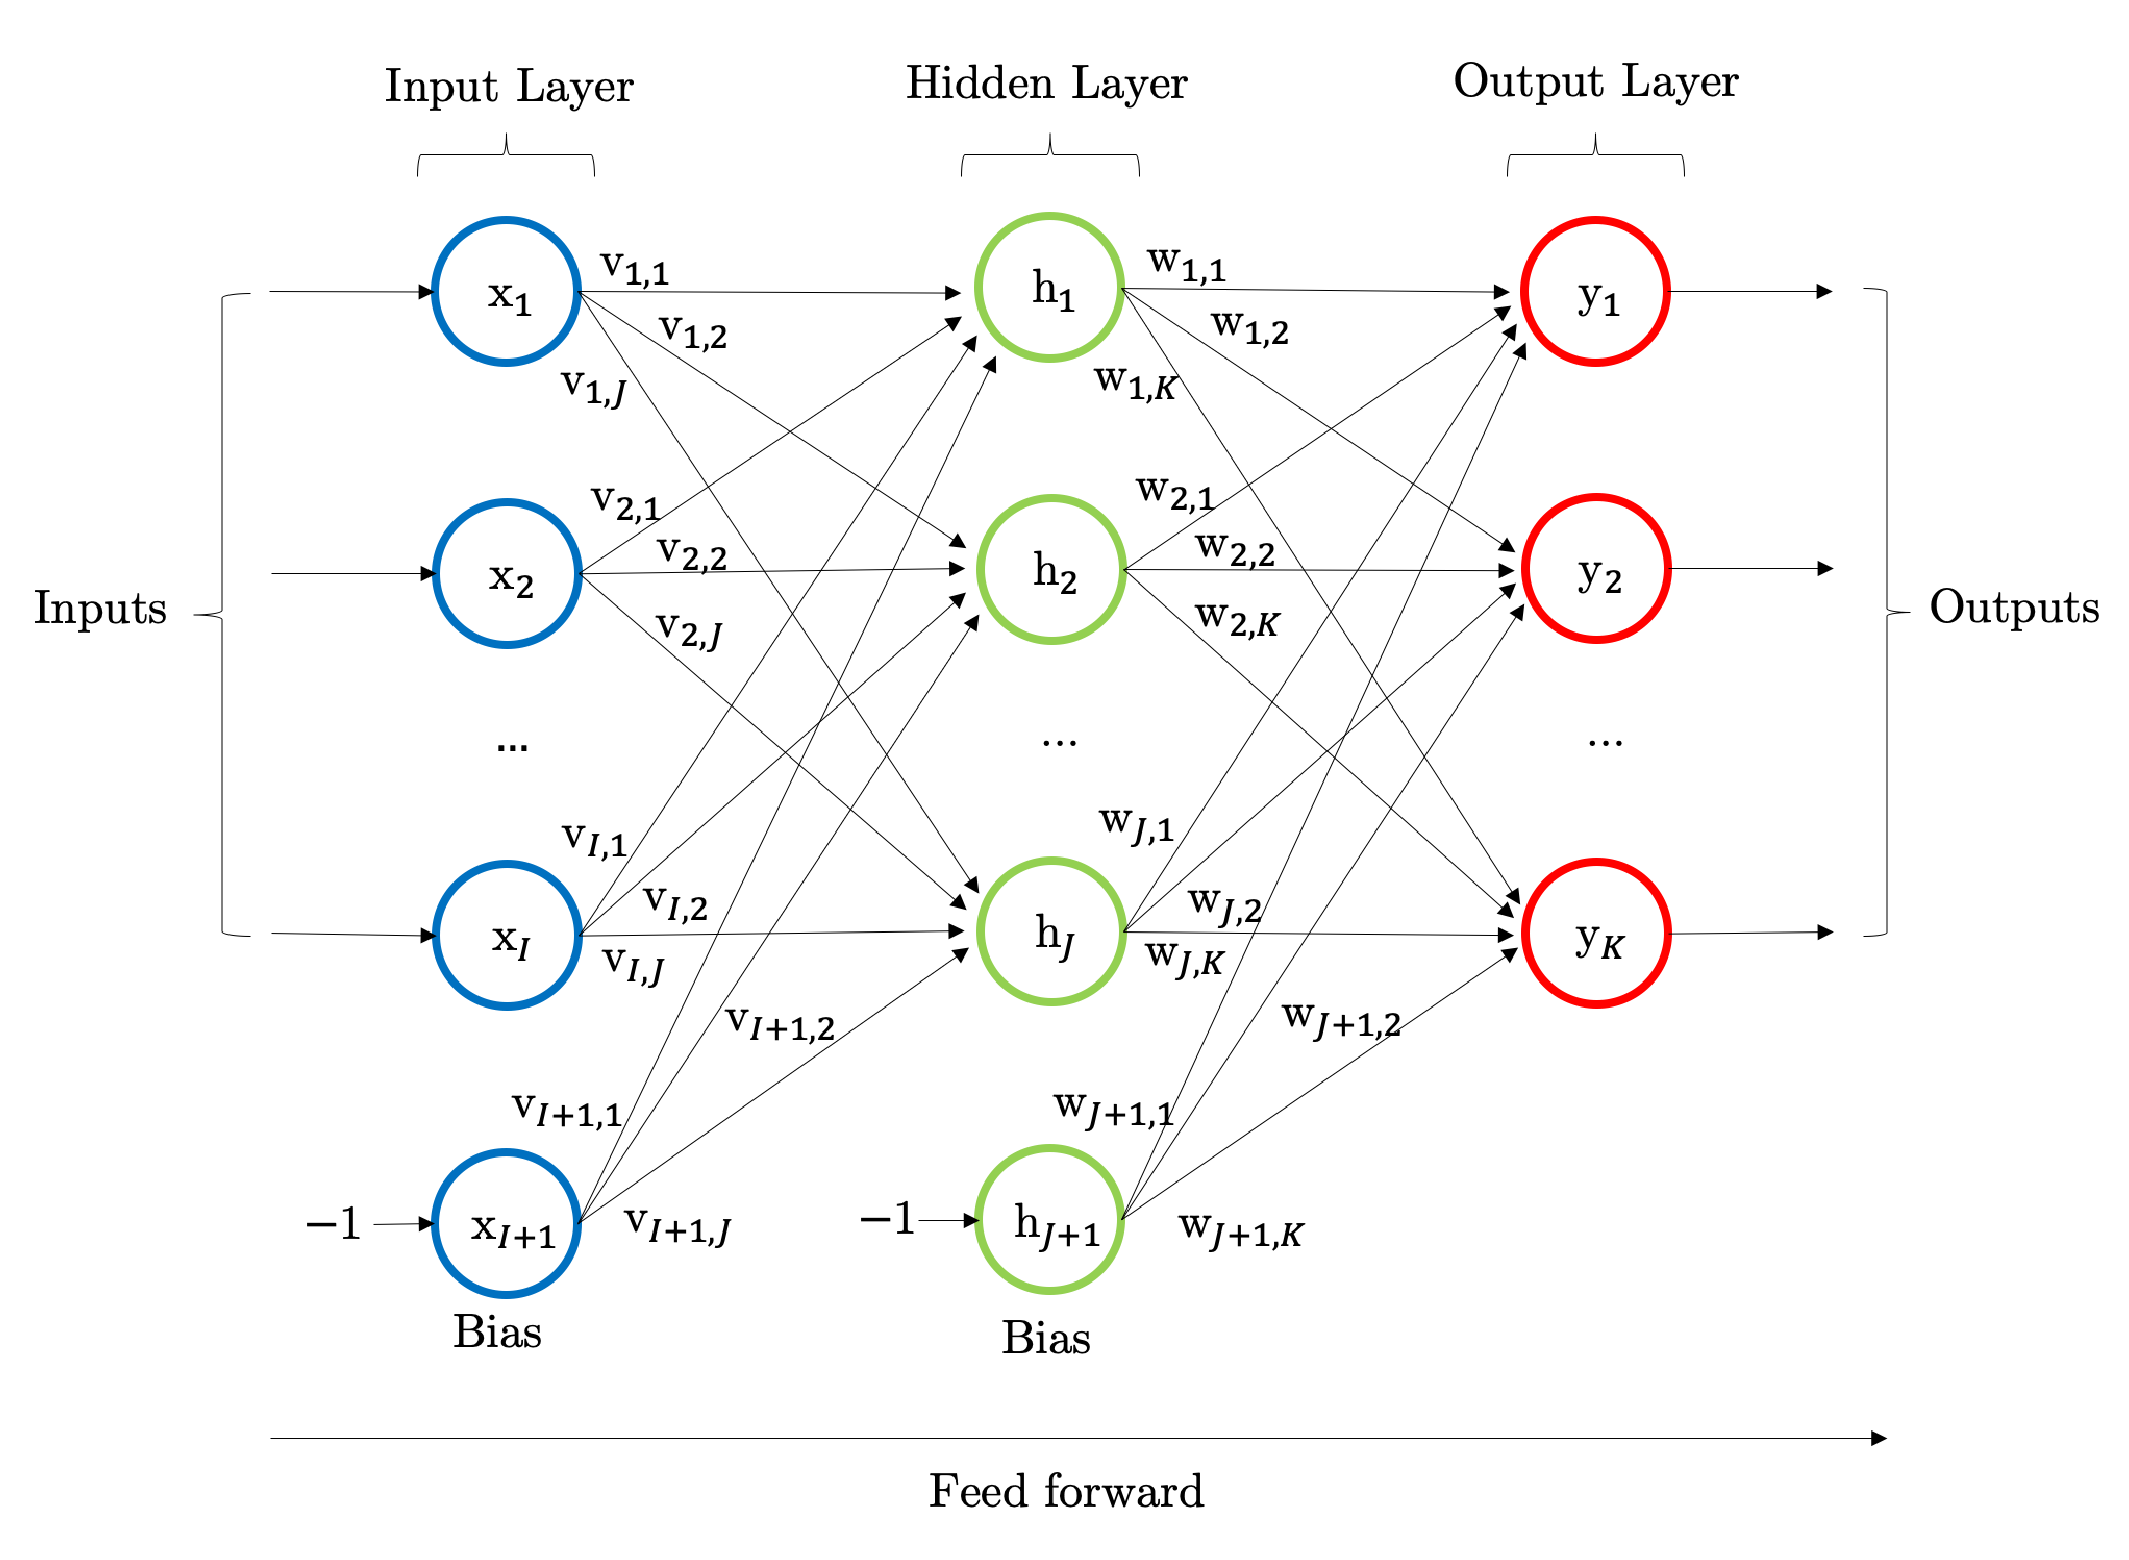
\includegraphics[width=0.8\textwidth]{feedforward_neural_network.eps}
    \caption[A \index{Feedforward Neural Network}Feedforward neural network]{An
    illustration of a \index{Feedforward Neural Network}feedforward neural network.}
    \label{fig:ffnn}
\end{figure}

In Figure~\ref{fig:ffnn}, $x_i$ refers to the $i$-th dimension in the input
vector $\vec{x}$, $h_j$ refers to the $j$-th dimension in the hidden layer,
$y_k$ refers to the $k$-th dimension in the output vector $\vec{y}$. $v_{i,j}$
refers to the weight associated with input node $x_i$ and the hidden node $h_j$
and $w_{j,k}$ refers to the weight associated with hidden node $h_j$ and the
output node $y_k$.

With the layered architecture and \index{fully connected topology}fully
connected topology of \acp{FFNN} and assuming the use of \acp{SU}, the output
for the \ac{FFNN} at index $k$, denoted $y_k$ is calculated using:

\begin{equation}
    \label{eq:ffnn}
    \begin{split}
        y_k &= f\left(net_{h,y}\right) \\
            &= f\left(\sum_{j=0}^{J+1} h_j w_{j,k}\right) \\
            &= f\left(\sum_{j=0}^{J+1} f\left(net_{i,h}\right) w_{j,k}\right) \\
            &= f\left(\sum_{j=0}^{J+1} f\left(\sum_{i=0}^{I+1} x_i v_{i,j}\right) w_{j,k}\right) \\ 
    \end{split}
\end{equation}

\noindent The remainder of this thesis makes use of \acp{FFNN} as the \ac{ANN}
of interest and is sometimes referred to as \textit{the model}.


\section{Training}
\label{sec:anns:training}

Section~\ref{sec:anns:an:weights} mentioned that changing the weight associated
with a feature, changes the influence of that particular feature on the
predicted output. \textit{Training} is the process whereby the weights of the
\acp{FFNN} is systematically changed with the aim of improving performance.

Finding the optimal weights that produce the best output is an optimisation
problem and therefore, training of \acp{FFNN} is done using a search function
called a \index{Heuristic}\textit{heuristic}. \index{Heuristic}Heuristics search
for possible solutions in the solution-space and make use of information from
the search-space to guide to process. Heuristics are discussed in detail in
Chapter~\ref{chap:heuristics}.

Details on the training of \acp{FFNN} is presented in this section along with
brief discussions on the training process, generalisation capabilities, training
sets, \index{Supervised Learning}supervised learning, error functions, and
performance measurement.

 
\subsection{Training Process}
\label{sec:anns:training:process}

During the training process, the \ac{FFNN} is exposed to input data while
trying to predict some expected outcome. From this prediction, a \textit{cost}
is calculated based on the degree to which the predicted output differs from the
expected outcome. This outcome could be predefined and static, or be the result
of an action in a dynamic environment. This cost is used by some
\index{Heuristic}heuristic as a guide to update the weights slightly such that
the performance of the \ac{FFNN} improves over time.

The training process is executed as follows: training data is retrieved and
pre-processed. The pre-processed input data is then split into various datasets.
A loss is calculated by exposing all patterns in the training data to the
\ac{FFNN} and evaluating the  prediction in comparison to the expected or target
output. Exposing the \ac{FFNN} to all training data once is referred to as an
epoch. The \ac{FFNN} is trained for a maximum number of epochs, or until some
stopping condition is reached. After training, the generalisation capabilities
of the \ac{FFNN} is evaluated against never before seen data.

Central to this thesis is the topic of generalisation. Generalisation refers to
the ability of a model to balance under- and overfitting of data. Training a
\ac{FFNN} using a \ac{HH} aims to do exactly that. Overfitting and underfitting
concepts are discussed next.

\subsubsection{Overfitting}
\label{sec:anns:training:overfitting}

\index{Overfitting}Overfitting describes a scenario where the trained model
performs well on training data, but does not generalise well to never before
seen data. \cite{ref:tetko:1995, ref:geron:2017}. Geron \cite{ref:geron:2017}
mentions that \index{overfitting}overfitting occurs when the model is too
complex relative to the noisiness of the training data.


\subsubsection{Underfitting}
\label{sec:anns:training:generalisation_capabilities:underfitting}

\index{underfitting}Underfitting is the opposite of
\index{overfitting}overfitting. Geron \cite{ref:geron:2017} mentions that
\index{underfitting}underfitting occurs when the model is too simple relative to
the underlying structure of the training data.


\subsection{Training Sets}
\label{sec:anns:training:sets}

The input data is split proportionally into a training and testing set. Data in
the training set is used to train the \ac{FFNN} \cite{ref:james:2013}, while the
generalisation capabilities of the \ac{FFNN} is evaluated over the performance
of the trained model when exposed to never before seen data in the testing set.
Some research propose a validation set whereby the trained model is evaluated on
the validation data while hyper-parameters are tuned \cite{ref:brownlee:2017}.


\subsection{Supervised Learning}
\label{sec:anns:training:supervised_learning}

\index{supervised learning}Supervised learning is the process of learning where
the training data that is presented to the \ac{FFNN} includes the desired
solution \cite{ref:geron:2017}.  The \ac{FFNN} learns the mapping function from
the input to the target output \cite{ref:brownlee:2016}. These desired solutions
are referred to as \textit{labels}. \index{supervised learning}Supervised
learning can be used for both classification and regression problems.

There are two types of supervised learning algorithms based on when weights are
updated \cite{ref:engelbrecht:2007}. These include stochastic training and batch
training and is discussed next.


\subsubsection{Stochastic Training}
\label{sec:anns:training:stochastic}

\index{Stochastic Training}Stochastic training, also known as \index{Online
Learning}\textit{online learning}, is a \index{Supervised Learning}supervised
learning variation whereby weights are adjusted after each training pattern is
presented.

If \index{stochasting training}stochastic training is used to train the
\ac{FFNN}, the training data must be shuffled before splitting into sets, in
order to avoid overfitting or memorising the order in which patterns are
presented in the training set \cite{ref:engelbrecht:2007}. It has been shown
that shuffling the training data can speed up convergence
\cite{ref:bengio:2012}. 


\subsubsection{Batch Training}
\label{sec:anns:training:batch}

\index{Batch Training}Batch training, also known as \index{Offline
Learning}\textit{offline learning} is a supervised training variation whereby
the weight changes are accumulated and used to adjust the weights once after all
the training patterns have been presented. 


\subsubsection{Mini-Batch Training}
\label{sec:anns:training:mini_batch}

Research suggests a trade-off between stochastic and batch training by making
use of mini-batches \cite{ref:bengio:2012}. Mini-batch training is the same as
batch training, however, weights are updated after $\beta$ patterns have been
presented, where $\beta$ is the batch size.


\subsection{Error Functions}
\label{sec:anns:training:error_functions}

An error function, also known as a \index{Loss Function}\index{Cost
Function}\textit{loss/cost function} \cite{ref:changhau:2017} is used to
evaluate the model's capability to approximate output data based on the input
patterns presented. It measures the degree to which the model is capable of
predicting the correct output data.  This error value is used by the
\index{Heuristics}heuristic as a guide during the training process.

This thesis focusses on the following error functions: \ac{SSE}, \ac{MSE},
\ac{RMSE}, \ac{MAE}, \ac{BinXE}, \ac{CatXE} and \ac{SparseCatXE}. Each of these
are discussed next.


\subsubsection{Sum Squared Error}
\label{sec:anns:training:error_functions:sse}

The \ac{SSE} is computed using:

\begin{equation}
    \epsilon = \sum_{p=1}^P \sum_{k=1}^K (\hat{y}_{k,p} - y_{k,p})^2
    \label{eq:sse}
\end{equation}

\noindent where $\hat{y}_{k,p}$ is $k$-th dimension of the target output of
pattern $p$, $y_{k,p}$ is $k$-th dimension of the predicted output vector
$\vec{y}_{p}$ for pattern $p$, $P$ is the number of patterns in the training
set, and $K$ is the number of dimensions in the output vector $\vec{y}$.


\subsubsection{Mean Squared Error}
\label{sec:anns:training:error_functions:mse}

The \ac{MSE} is computed using:

\begin{equation}
    \epsilon = \frac{\sum_{p=1}^P \sum_{k=1}^K (\hat{y}_{k,p} - y_{k,p})^2}{PK}
    \label{eq:mse}
\end{equation}


\subsubsection{Root Mean Squared Error}
\label{sec:anns:training:error_functions:rmse}

The \ac{RMSE} is computed using:

\begin{equation}
    \epsilon = \sqrt{\frac{\sum_{p=1}^P \sum_{k=1}^K (\hat{y}_{k,p} - y_{k,p})^2}{PK}}
    \label{eq:rmse}
\end{equation}


\subsubsection{Mean Absolute Error}
\label{sec:anns:training:error_functions:mae}

The \ac{MAE} is computed using:

\begin{equation}
    \epsilon = \frac{\sum_{p=1}^P \sum_{k=1}^K |\hat{y}_{k,p} - y_{k,p}|}{PK}
    \label{eq:mae}
\end{equation}


\subsubsection{Binary Cross-Entropy}
\label{sec:anns:training:error_functions:bin_xe}

\noindent The \ac{BinXE} is computed using:

\begin{equation}
    \epsilon = -\frac{\sum_{p=1}^P \sum_{k=1}^K (\hat{y}_{k,p} \log{(y_{k,p})} + (1 - \hat{y}_{k,p})\log{(1 - y_{k,p})})}{PK}
    \label{eq:bin_xe}
\end{equation}

\noindent \ac{BinXE} is used in classification problems, where there are only
two classes in the target output data.


\subsubsection{Categorical Cross-Entropy}
\label{sec:anns:training:error_functions:cat_xe}

The \ac{CatXE} is computed using:

\begin{equation}
    \epsilon = -\frac{\sum_{p=1}^P \sum_{k=1}^K \sum_{c=1}^C (\mathbbm{1}_{\hat{y}_{k,p} \in C_c} \log{(y_{k,p} \left[ y_{k,p} \in C_c \right])})}{PK}
  \label{eq:cat_xe}
\end{equation}

\noindent where $\mathbbm{1}$ is the indicator function that the $k$-th index observation
belongs to the $c$-th class. $C$ is the total number of unique class labels. If
$C = 2$, then \ac{BinXE} can be used instead.

\ac{CatXE} is used in classification problems where the target
output or \textit{label} is a one-hot encoded vector.


\subsubsection{Sparse Categorical Cross-Entropy}
\label{sec:anns:training:error_functions:sparse_cat_xe}

The \ac{SparseCatXE} error function is the same as \ac{CatXE} with the only
difference being that the target output or label is a one-hot
embedding of a class represented as an integer, $c \in \{1,2, \dots, C\}$.


\subsection{Performance Measures}
\label{sec:anns:training:performance_measures}

Performance measures play an important role in understanding how well a
\ac{FFNN} has been trained to predict target output. Performance metrics are
used during training on the training set and evaluation on the test set. These
performance metrics provide a mechanism by which different implementations of
\acp{FFNN} and training processes can be compared.

There are many different mechanisms that can be used to measure the performance
of a \ac{FFNN}, however this thesis only focusses on measures of cost such as
loss and speed. Brief discussions follow on loss and speed as performance
measures.

\subsubsection{Loss/Cost}
\label{sec:anns:training:performance_measure:loss_cost}

A measure of cost indicates how well the \ac{FFNN} is able to predict target
output and often include a metric over some distance between the predicted
output and target output. This metric is calculated using an error function as
described in Section~\ref{sec:anns:training:error_functions}.

In the case of classification problems, the loss/cost can be expressed in terms
of \textit{accuracy}. Accuracy refers to the percentage of patterns for which
the \ac{FFNN} was able to successfully predict the target output. 

\subsubsection{Speed}
\label{sec:anns:training:performance_measure:speed}

Speed is a performance measure which calculates how fast a \ac{FFNN} can reach
some target goal. Speed is often expressed relative to another performance
measurement metric e.g how many epochs of training is necessary for a \ac{FFNN}
to reach a certain lost/cost threshold. If emperical tests run on simular
enviroments, relative time of execution can be used, but this is less popular.

For this thesis, speed is a measure of performance relative to training
\textit{steps} or \textit{mini-batch} steps.


\subsection{Stopping Conditions}
\label{sec:anns:training:stopping_conditions}

Stopping conditions are required to stop the training process. The goal of the
stopping condition is to try and stop the training process to avoid unnecessary
computational cost or to set a comparible timeframe in which \acp{FFNN} are
trained. Stopping conditions include:

\begin{itemize}
    \item
    \textbf{Max Epochs}: Stop when a maximum number of epochs has been reached.

    \item
    \textbf{Performance Measurement Threshold}: Stop the training when the
    performance measurement metric has reached some acceptable threshold.

    \item
    \textbf{Stagnation}: Stop the training process if no improvements in the
    performance of the model is observed over a window of epochs.

    \item
    \textbf{Overfit}: Stop the training process if the generalisation on the
    test set indicates that the \ac{FFNN} is overfitting the data.
\end{itemize}


\section{Summary}
\label{sec:anns:summary}

This chapter presented background information on the \ac{BN} and it was shown
how neurons connect to each other. Emphasis was put on \index{Synapse}synapses
and how communication happens between neurons. The \ac{AN} was introduced in
Section~\ref{sec:anns:an} and it was shown how the brain inspired the
development of \acp{AN}. Brief discussions followed on the various components
that make up the \ac{AN}. Details on input, weights, \index{net input signal}net
input signal, biases, \index{activation function}activation functions, and
output were provided.  Section~\ref{sec:anns:ann} introduced \acp{ANN}. It was
shown how \acp{AN} are connected together to form networks. \ac{ANN} design was
described in terms of architecture and topologies. Special emphasis was put on
\acp{FFNN} as the model being used throughout the rest of the thesis.
Section~\ref{sec:anns:training} provided the necessary background information
required on the training of \acp{FFNN}. It is emphasised that the training of an
\ac{ANN} is an optimisation problem where optimal values for weights and biases
are sought such that a given cost function is minimised. The training process
was explained and details on training sets was provided. A variant of learning,
called \index{Supervised Learning}supervised learning is presented and led to
the discussion on error functions, performance measures, and stopping
conditions.

Chapter~\ref{chap:heuristics} introduces background information on optimisation
and heuristics. 

